\fenicschapter{Lessons learned in mixed language programming}
              {Mixed Language Programming}
              {Johan Hake and Kent-Andre Mardal}
              {mardal-2}


This chapter describes decisions made and lessons learnt
in the implementation of PyDOLFIN. The chapter is quite technical, since
we aim at giving the reader a thorough understanding of the implementation
of PyDOLFIN. 

\section{Background}
Python has over the last decade become an established platform
for scientific computing. Widely used scientific software such as, e.g.,
\citet{www:petsc}, \citet{www:hypre},
\citet{www:trilinos}, \cite{www:vtk}, \cite{www:vmtk},
\ginac~\citep{BauerFrinkKreckel2000} have all been equipped with Python
interfaces. The \fenics
packages \ferari, \fiat , \ffc,
\ufl, \viper, as well as  other packages such as 
\sympy\citep{CertikSeoanePetersonEtAl2009},
\scipy\citep{JonesOliphantPetersonEtAl2009} are pure Python packages.
The \dolfin library has both a C++ and a Python user-interface. Python
makes application building on top of \dolfin more user friendly, but
the Python interface also introduces additional complexity and new
problems.  We assume that the reader has basic knowledge of both C++
and Python. A suitable textbook on Python for scientific computing is
\cite{Langtangen2008}, which cover both Python and its C interface.
SWIG is well documented and we refer to the user manual that can be
found on its web page~\cite{www:swig}. Finally, we refer to
\citet{Langtangen2003b} and \citet{SalaSpotzHeroux2008} for a
description of how SWIG can be used to generate Python interfaces for
the other packages Diffpack and Trilinos.


\section{Using SWIG}

Python and C++ are two very different languages, while Python is
user--friendly and flexible, C++ is very efficient. 
To combine the strengths of the two languages, it has become common
to equip C++ (or FORTRAN/C) libraries with Python interfaces. 
Such interfaces must comply the \citet{www:python-capi}.   
Writing such interfaces, often called wrapper code, is quite involved.
Therefore, a number of wrapper code generators have been developed in the
recent years, some examples are   
 \citet{Peterson}, \citet{SIP}, \citet{Siloon}, and \citet{www:swig}. 
 SWIG has been used to create PyDOLFIN and will therefore be in focus in
 this chapter. SWIG is a mature wrapper code generator that support many languages and is extensively documented.

\subsection{Basic SWIG}
To get a basic understanding of SWIG, we consider  an implementation of an array class. 
Let the array class be defined in \emp{Array.h} as follows:
\lstinputlisting[style=mycpp]{chapters/mardal-2/code/Array.h}
A first attempt to make the Array accessible in Python using SWIG, is to write a SWIG interface file \emp{Array\_1.i}.
\lstinputlisting[style=mycpp]{chapters/mardal-2/code/Array_1.i}
Here, we specify the name of the Python module: \emp{Array}; the code
that should be inlined in the wrapper code directly (the declarations):
\emp{\#include "Array.h"}; and the code SWIG should parse to create the wrapper code: \emp{\%include "Array.h"} (definitions). The following command shows how to run SWIG to produce the wrapper code:
\begin{bash}
swig -python -c++ -I. -O Array_1.i
\end{bash}
The command generates two files: \emp{Array.py} and
\emp{Array\_}\emp{wrap.cxx}. The file
\emp{Array\_}\emp{wrap.cxx} contains C code that defines the Python
interface of Array.  After \emp{Array\_wrap.cxx} is compiled into a
shared library, it can be imported into Python. 
The file \emp{Array.py} is written in pure Python.  It imports the shared library and may add some
functionality to the Python module. 
The reader should be able to recognize the Python class \emp{Array} at the end of the \emp{Array.py} file. 

The following \citet{www:distutils} file (\emp{setup.py}) executes the SWIG command above and compiles and links the source code and the generated wrapper code into a shared library.
\lstinputlisting[style=mypython]{chapters/mardal-2/code/setup.py}
Build and install the module in the current working directory with the
command:
\begin{bash}
python setup.py install --install-lib=.
\end{bash}

The Python proxy class resembles the C++ class in many ways. Simple methods
such as \emp{dim()} and \emp{norm()} will be wrapped correctly to
Python, since SWIG maps \emp{int} and \emp{double} arguments to the
corresponding Python types through built-in typemaps.  
However, a number of issues appear:
\begin{enumerate}
\item the \emp{operator[]} does not work;
\item the \emp{operator+=} returns a new Python object (with different \emp{id});
\item printing does not use the \emp{std::ostream \& operator<<};%>> Put here so emacs highlighting wont go bananas
\item the \emp{Array(int n\_, double* a\_);} constructor is not working properly.%  neither is the overloading of the same method working.
\end{enumerate}
We see that a number of different problems arise even in such a simple
example. Fortunately, these problems are fairly common, and general
solutions can be implemented quite easily. In the following, we will go through 
each of the above issues. The example code with the solutions proposed in
the following can be found in \emp{Array\_2.i}. 

\subsection{The \emp{operator[]}}
In C++ the subscripting \emp{operator[]} is used to implement both set and get
operators. It is possible to distinguish the set operator from the get
operator using \emp{const}, but this is not required.  
In Python subscripting is performed with the two special methods: \emp{\_\_setitem\_\_} and \emp{\_\_getitem\_\_}. 
Since, the mapping between the Python operators 
(\emp{\_\_setitem\_\_} and \emp{\_\_getitem\_\_}) and the C++ operators \emp{operator[]} 
may be ambiguous, SWIG currently ignores these operators. 
To implement the operators properly, also in future versions of SWIG, we ignore both version of the \emp{operator[]} with
\begin{c++}
%ignore Array::operator[];
\end{c++}
and extend the interface with the auxiliary 
\emp{\_\_setitem\_\_} and \emp{\_\_getitem\_\_} methods: 
\begin{c++}
%extend Array {
double __getitem__(int i) {
  return (*self)[i];
}

void __setitem__(int i, double v) {
  (*self)[i] = v;
}
...
};
\end{c++}
Note that all SWIG directives start with '\emp{\%}'.
Furthermore, the access to the actual instance is provided by the
\emp{self} pointer, which in this case is a C++ pointer that points to an
\emp{Array} instance. The pointer is comparable to the \emp{this} pointer
in a C++ class, but only the public attributes are available. 

%A basic observation here is that Python does not have \emp{const} types. This means that if SWIG would have wrapped the \emp{operator[]} methods in the \emp{Array} class ...
\subsection{\emp{operator +=}}
The second problem is related to SWIG and garbage collection in Python.
Python features garbage collection, which means that a user should not be
concerned with the destruction of objects. The mechanism is based on
reference counting; that is, when no more references are pointing to an
object, the object is destroyed. The SWIG generated Python module consists
of a small Python layer that defines the interface to the underlying C++
object. An instance of a SWIG generated class therefore keeps a reference
to the underlying C++ object. The default behavior is that the C++ object is destroyed together 
with the Python object. This behavior is not consistent with the
\emp{operator +=} returning a new object, which is illustrated 
by the segmentation fault in the following example 
(see \emp{segfault\_test.py}):
\lstinputlisting[style=mypython]{chapters/mardal-2/code/segfault_test.py}
This script produces the following output:
\begin{python}
id(a): 3085535980
id(b): 3085535980
id(b): 3085536492
Segmentation fault
\end{python}
The script causes a segmentation fault because the underlying C++ object is
destroyed after the call to \emp{add()}. When the last \emp{a+=a} is
performed the underlying C++ object is already destroyed. This happens
because the SWIG generated \emp{\_\_iadd\_\_} method returns a new Python
object. This is illustrated by the different values obtained from the
\emp{id()} function\footnote{Taking \emp{id} of a Python object returns a
unique reference to that object.}. The last two calls to \emp{id(b)}
return different numbers, which means that a new Python object is
returned by the SWIG generated \emp{\_\_iadd\_\_} method. The second
\emp{b} object is local in the \emp{add} function and 
is therefore deleted together with the underlying C++ object when \emp{add} has finished.  

The memory problem can be solved by extending the interface with
an \emp{\_add} method and implementing our own \emp{\_\_iadd\_\_} method in
terms of \emp{\_add}, using the \emp{\%extend} directive:
\begin{c++}
%extend Array {
...
  void _add(const Array& a){
    (*self) += a;
  }

  %pythoncode %{
    def __iadd__(self,a):
      self._add(a)
      return self
  %}
...
};
\end{c++}
The above script will now report the same \emp{id} for all objects. 
No objects are created or deleted, and segmentation fault is avoided.

\subsection{ \emp{std::ostream \& operator<<}}%>>
In C++, shift operators such as \emp{operator <<} are typically used to implement I/O, while in
Python the \emp{\_str\_} method is used.    
Therefore, SWIG ignores the shift operator, as it is likely not to perform as intended. 
However, we can again use the \emp{\%extend} directive to make this
operator available from Python by adding a  \emp{\_\_str\_\_} method.
\begin{c++}
%include <std_string.i>

%extend Array {
...
  std::string __str__() {
    std::ostringstream s;
    s << (*self);
    return s.str();
  }
};
\end{c++}
This method uses the \emp{operator<<} %>>
to pipe the stream representation of the array to a
\emp{std::ostringstream} and then returns a \emp{std::string}
representation of the stream.
Note that we need to include \emp{std\_string.i} in the \emp{Array\_2.i}.
In Python, we can then call \emp{print} on an instance of \emp{Array}.

\subsection{The constructor: \emp{Array(int n\_, double* a\_);}}
The fourth problem is related to pointer handling in C/C++ and SWIG. From
the constructor signature alone, it is not clear whether \emp{double* a\_} points to a single value or to the first element of an array.
Therefore, SWIG takes a conservative approach and handles pointers as
pointers. This leads to the erroneous behaviour of the constructor in the
above example, where  \emp{double* a\_} points to the first element of an array of length \emp{n}. 
As a remedy, SWIG provides the \emp{typemap} concept to enable mappings
between C/C++ and Python types. The following code, explained in detail
below, demonstrates how to map a \numpy array to the \emp{(int n\_, double* a\_)} 
arguments in the constructor.
\begin{c++}
%typemap(in) (int n_, double* a_){
  if (!PyArray_Check($input)) {
    PyErr_SetString(PyExc_TypeError, "Not a NumPy array");
    return NULL; ;
  }
  PyArrayObject* pyarray = reinterpret_cast<PyArrayObject*>($input);
  if (!(PyArray_TYPE(pyarray) == NPY_DOUBLE)) {
    PyErr_SetString(PyExc_TypeError, "Not a NumPy array of doubles");
    return NULL; ;
  }
  $1 = PyArray_DIM(pyarray,0);
  $2 = static_cast<double*>(PyArray_DATA(pyarray));
}
\end{c++}
The first line specifies that the typemap should be applied to the input
\emp{(in)} arguments of operators, functions, and methods with 
\emp{int n\_,double* a\_} arguments in the signature. 
The \$ prefixed variables are used to map input and output variables in the typemap; 
that is, the variables \$1 and \$2 map to the first and second output C
arguments of the typemap, \emp{n\_} and \emp{a\_}, while \emp{\$input}
maps to the Python input. 

In the next three lines, we check that the input Python object is a \numpy array, and raise an exception if not.
Note that any Python C-API function that returns \emp{NULL} tells the
Python interpreter that an exception has occurred. Python will then raise
an error, with the error message set by the \emp{PyErr\_SetString}
function. Next, we cast the Python object pointer to a \numpy array pointer
and check that the data type of the \numpy array is correct; that is, that it contains doubles. Then, we acquire the data from the \numpy array and assign the two input variables.

Overloading operators, functions and methods is not possible in Python.
Instead, Python dynamically determines what code to call,  
a process which is called dynamic dispatch.
To generate proper wrapper code, 
SWIG relies on \emp{\%typecheck} directives to resolve the overloading. 
A suitable typecheck for our example typemap is:
\begin{c++}
%typecheck(SWIG_TYPECHECK_DOUBLE_ARRAY) (int n_, double* a_) {
   $1 = PyArray_Check($input) ? 1 : 0;
 }
\end{c++}
Here, \emp{SWIG\_TYPECHECK\_DOUBLE\_ARRAY} is a \emp{typedef} for the priority number assigned for arrays of doubles. The typecheck should return 1 if the Python object \emp{\$input} has the correct type, and 0 otherwise.
\section{SWIG and PyDOLFIN}
To make PyDOLFIN more \textit{Pythonic}, we have made a number of
specializations, along the lines mentioned above, that we will now go
through. But let us start with the
overall picture.   
The interface files resides in the \emp{dolfin/swig} directory, and are
organized into \textit{i)} global files, that apply to the entire \dolfin
library, and \textit{ii)} kernel module files that apply to specific
\dolfin modules. The latter files are divided into \emp{$\ldots$\_pre.i}
and \emp{$\ldots$\_post.i} files, which are applied before and after the
inclusion of the header files of the particular kernel module, respectively. 
The kernel modules (\emp{kernel\_module.i} mirror the structure of \dolfin: \emp{common}, \emp{parameters}, \emp{la}, \emp{mesh} and so forth. The global interface files are all included in \emp{dolfin.i}, the main SWIG interface file. The kernel module interface files are included, together with the C++ header files, in the automatically generated \emp{kernel\_modules.i} file.

The following sections deal with the main
interface file of \emp{dolfin.i} and address the global interface files. Then we will address some issues in the module specific interface files.

\subsection{\emp{dolfin.i} and the \emp{cpp} module}
The file \emp{dolfin.i} starts by defining the name of the generated Python module.
\begin{c++}
%module(package="dolfin", directors="1") cpp
\end{c++}
This statement tells SWIG to create a module called \emp{cpp} that resides
in the package of \emp{dolfin}. We have also enabled the use of directors.
The latter is required to be able to subclass \dolfin classes in Python,
and issue that will be discussed below.  By naming the generated extension module
\emp{cpp}, and including it in the \emp{dolfin} Python package, we hide the generated interface into a sub module of dolfin; the \emp{dolfin.cpp} module. 
The \emp{dolfin} module then imports the needed classes and functions 
from \emp{dolfin.cpp} in the \emp{\_\_init\_\_.py} file along with  pure Python classes and functions. 

The next two blocks of \emp{dolfin.i} defines code that will be inserted into the SWIG generated C++ wrapper file.
\begin{c++}
%{
#include <dolfin/dolfin.h>
#define PY_ARRAY_UNIQUE_SYMBOL PyDOLFIN
#include <numpy/arrayobject.h>
%}

%init%{
import_array();
%}
\end{c++}
SWIG inserts code that resides in a \emp{\%\{$\ldots$\}\%} block, verbatim
at the top of the generated C++ wrapper file. Note that
\emp{\%\{$\ldots$\}\%} is short for \emp{\%header\%\{$\ldots$\}\%}. Hence,
the first block of code is similar to the include statements you would
put in a standard C++ program. The code in the second block,
\emp{\%init\%\{$\ldots$\}\%}, is inserted in the code where the Python
module is initialized. A typical example of such a function is
\emp{import\_array()}, which initialize the \numpy module. SWIG provides
several such statements, each inserting code verbatim into the wrapper file
at different positions.


\subsection{Reference counting using shared\_ptr}
In the previous example dealing with \emp{operator+=}, we saw that it is
important to prevent premature destruction of underlying C++ objects. A
nice feature of SWIG is that we can declare that a wrapped class shall
store the underlying C++ object using a shared pointer \emp{shared\_ptr}, instead of a raw
pointer. By doing so, the underlying C++ object is not explicitly deleted
when the reference count of the Python object reach zero, instead the
reference count on the \emp{shared\_ptr} is decreased. \dolfin provides a
\emp{shared\_ptr} interface for some crucial classes, which interact
seamlessly with the \emp{shared\_ptr} stored C++ objects in \dolfin. 

Shared pointers are provided by the the \emp{boost\_shared\_ptr.i} file. 
This file declares two user macros: \emp{SWIG\_}\-\emp{SHARED\_}\-\emp{PTR}
and \emp{SWIG\_}\-\emp{SHARED\_PTR\_}\-\emp{DERIVED}\footnote{In SWIG
version 2.0 and above, these macros are superseeded by the single
\emp{\%shared\_ptr} directive.}. These macros must be called for each class we
want shared pointers.  In PyDOLFIN this is done in the \emp{shared\_ptr\_classes.i} file. 
Note that the macros also declare typemaps for passing a
\emp{shared\_ptr} stored object to method that expects a reference or
a pointer. This means that the typemap pass a
de-referenced \emp{shared\_ptr} to the function. This behavior can lead to
unintentional trouble because the \emp{shared\_ptr} mechanism is circumventeded.

In \dolfin, instances of some crucial classes are stored internally with
\emp{shared\_ptr}s. These classes also uses \emp{shared\_ptr} in the Python
interface. When objects of these classes are passed as arguments to methods
or constructors in \dolfin, two versions are needed: a \emp{shared\_ptr} and a reference version. The following code snippet illustrates two constructors of \emp{Function}, each taking a \emp{FunctionSpace} as an argument\footnote{Instances of \emp{FunctionSpace} are stored using \emp{shared\_ptr} in the \dolfin C++ library.}:
\begin{c++}
/// Create function on given function space
explicit Function(const FunctionSpace& V);

/// Create function on given function space (shared data)
explicit Function(boost::shared_ptr<const FunctionSpace> V);
\end{c++}
Instances of \emp{FunctionSpace} in PyDOLFIN are stored using
\emp{shared\_ptr}. Hence, we want SWIG to use the second constructor. However, 
SWIG generates de-reference typemaps for the first constructor. So when a
\emp{Function} is instantiated with a \emp{FunctionSpace}, SWIG will
unfortunately pick the first constructor and the \emp{FunctionSpace} is
passed without increasing the reference count of the \emp{shared\_ptr}.
This undermines the whole concept of \emp{shared\_ptr}. To prevent this
faulty behavior, we ignore the reference constructor (see \emp{function\_pre.i}):
\begin{c++}
 %ignore dolfin::Function::Function(const FunctionSpace&);
\end{c++}

\subsection{Typemaps}
Most types in the \emp{kernel\_module.i} file are wrapped nicely
with SWIG. However, as in the \emp{Array} example above, there is need for 
typemaps, for instance to handle \numpy arrays.  
In \emp{dolfin.i} we include three different types of global typemaps:
\textit{i)} general-, \textit{ii)} \numpy- and, \textit{iii)}
std\_vector-typemaps. These are implemented in the interface files:
\emp{typemaps.i}, \emp{numpy\_}\emp{typemaps.i} and
\emp{std\_}\emp{vector\_}\emp{typemaps.i}. Here, we present some of the typemaps defined in these files.

In \emp{typemaps.i}, typemaps for four different basic types are defined. In- and out-typemaps for \emp{dolfin::uint}, and \emp{dolfin::real}, an in-typemap for \emp{int}, and an out-typemap macro for \emp{std::pair<}\-\emp{dolfin::uint,}\-\emp{dolfin::uint>}.

The simplest typemap is an out-typemap for \emp{dolfin::uint}, which is needed since Python does not have \emp{unsigned int}:
\begin{c++}
%typemap(out) dolfin::uint = int;
\end{c++}
This typemap specifies that a function returning a \emp{dolfin::uint}
should use the built-in out-typemap for \emp{int}. SWIG lets us reuse a
typemap by simply copying it. We could have used the same feature for the
corresponding in-typemap, however an unfortunate bug, explained below,  
forces us to implement the whole typemap from scratch. The typemap looks like this:
\begin{c++}
%typemap(in) dolfin::uint
{
  if (PyInteger_Check($input))
  {
    long tmp = static_cast<long>(PyInt_AsLong($input));
    if (tmp>=0)
      $1 = static_cast<dolfin::uint>(tmp);
    else
      SWIG_exception(SWIG_TypeError, "expected positive 'int' for argument $argnum");
  }
  else
    SWIG_exception(SWIG_TypeError, "expected positive 'int' for argument $argnum");
}
\end{c++}
%$ to fool emacs highlight...
The typemap has the same structure as the \numpy typemap above. We first
check that the object is of integer type, with the
\emp{PyInteger\_}\emp{Check} function. Here, we have implemented the
\emp{PyInteger\_}\emp{Check} function ourselves instead of using the 
Python  macro \emp{PyInt\_Check}. The reason is that
\emp{PyInt\_Check} can not be combined with \numpy, which is the above
mentioned bug. Next, we convert the Python integer to a \emp{long} and
check whether it is positive. Finally, we assign the input argument \$1 to
a \emp{dolfin::uint} casted version of the value. If either of these checks
fail, we use the built in SWIG function, \emp{SWIG\_exception} to raise a
Python exception. These predefined SWIG exceptions are defined in the
\emp{exception.i} file, included in \emp{dolfin.i}. Note that SWIG expands
the \emp{\$argnum} variable to the number of the argument using
the  \emp{dolfin::uint} typemap. Including this number in the string
creates  more understandable error message. 
%Finally, we define a corresponding typecheck for the typemap, which is not shown here. 
%After the \emp{dolfin::uint} typemap we also define an in-typemap for the \emp{int} type, 
%which is almost a copy of the \emp{uint} typemap and therefore not presented here.
Finally, we present the out-typemap for
\emp{std::pair}\-\emp{<dolfin::uint,}\-\emp{dolfin::uint>},  
which returns a Python tuple of two integers:\begin{c++}
%typemap(out) std::pair<dolfin::uint,dolfin::uint>
{
  $result = Py_Build Value("ii",$1.first,$1.second);
}
\end{c++}
%$ here to fool emacs highlightings
This is an example of a short and comprehensive typemap. It uses the Python C-API function \emp{Py\_BuildValue} to build a tuple of the two values in the \emp{std::pair} object.

In \emp{numpy\_typemaps.i}, typemaps for arrays of primitive types:
\emp{double}, \emp{int} and \emp{dolfin::uint} are defined. 
As in the \emp{Array} example above, these typemaps are defined so a \numpy
array of the corresponding type can be passed as the argument to functions,
methods, and operators. 
Instead of writing one typemap for each primitive type, we defined a SWIG
macro, which is called with different types as argument. Using macros may
produce a lot of code as some of these typemaps are used frequently. To
avoid code bloat, most of the typemap code is place in the function
\emp{convert\_numpy\_to\_}, which is called
by typemap. The entire macro reads:
\begin{c++}
%define UNSAFE_NUMPY_TYPEMAPS(TYPE,TYPE_UPPER,NUMPY_TYPE,TYPE_NAME,DESCR)
%{
SWIGINTERN bool convert_numpy_to_ ## TYPE_NAME ## _array_no_check(PyObject* input, TYPE*& ret)
{
  if PyArray_Check(input)
  {
    PyArrayObject *xa = reinterpret_cast<PyArrayObject*>(input);
    if ( PyArray_TYPE(xa) == NUMPY_TYPE )
    {
      ret  = static_cast<TYPE*>(PyArray_DATA(xa));
      return true;
    }
  }
  PyErr_SetString(PyExc_TypeError,"numpy array of 'TYPE_NAME' expected. Make sure that the numpy array use dtype='DESCR'.");
  return false;
}
%}

%typecheck(SWIG_TYPECHECK_ ## TYPE_UPPER ## _ARRAY) TYPE *
{
    $1 = PyArray_Check($input) ? 1 : 0;
}

%typemap(in) TYPE *
{
if (!convert_numpy_to_ ## TYPE_NAME ## _array_no_check($input,$1))
    return NULL;
}

%apply TYPE* {TYPE* _array}
%enddef
\end{c++}
The first line defines the signature of the macro. The macro is called using 5 arguments:
\begin{enumerate}
\item \emp{TYPE} is the name of the primitive type. Examples are 
\emp{dolfin::uint} and \emp{double}.
\item \emp{TYPE\_UPPER} is the name of the typecheck-name SWIG uses. Examples
are \emp{INT32} and \emp{DOUBLE}.
\item \emp{NUMPY\_TYPE} is the name of the \numpy type. Examples are
\emp{NPY\_UINT} and \emp{NPY\_DOUBLE}.
\item \emp{TYPE\_NAME} is a short typename used in exception string.
Examples are \emp{uint} and \emp{double}.
\item \emp{DESCR} is a description character used in \numpy to describe the
type. Examples are \emp{'I'} and \emp{'d'}.
\end{enumerate}
We can then call the macro to instantiate the typemaps and typechecks.
\begin{c++}
UNSAFE_NUMPY_TYPEMAPS(dolfin::uint,INT32,NPY_UINT,uint,I)
UNSAFE_NUMPY_TYPEMAPS(double,DOUBLE,NPY_DOUBLE,double,d)
\end{c++}
Here, we have instantiated the typemap for a \emp{dolfin::uint} and a
\emp{double} array. The above typemap does not check the length of the handed \numpy array 
and is therefore unsafe. Corresponding safe typemaps can also be found in
\emp{numpy\_typemaps.i}. 
The typemap function in the third line of the typemap
\begin{c++}
  SWIGINTERN bool convert_numpy_to_ ## TYPE_NAME ## _array_no_check(PyObject* input, TYPE*& ret)
\end{c++}
takes a pointer to a \emp{PyObject} as input. This function returns
\emp{true} if the conversion is successful and \emp{false} otherwise. The
converted array will be returned by the \emp{TYPE*\& ret} argument. 
Finally, the \emp{\%apply TYPE* \{TYPE* \_array\}} directive means that we want the typemap to apply to any argument of type \emp{TYPE*} with argument name \emp{\_array}. This is another way of copying a typemap, similar to what we did for the \emp{dolfin::uint} out-typemap above.

In \emp{std\_vector\_typemaps.i}, two typemap macros for passing
\emp{std::vector<Type>} between Python and C++ are defined. One is an
in-typemap macro for passing a std::vector of pointers of \dolfin objects
to a C++ function. The other is an out-typemap macro for passing a
\emp{std::vector} of primitives, using \numpy arrays, to Python. It is not
strictly necessary to add these typemaps as SWIG provides a
\emp{std::vector} type. However, the SWIG \emp{std::vector} functionality
is not very Pythonic and we have therefore chosen to implement our own typemaps to handle \emp{std::vector} arguments.

The first typemap macro enables the use of a Python list of \dolfin objects
instead of a \emp{std:vector} of pointers to such objects. Since  the
handed \dolfin objects may and may not be stored using a \emp{shared\_ptr},
we provide a  typemap that works for both situations. 
We also create typemaps for signatures where \emp{const} are used. 
Typically a signature can look like:
\begin{c++}
{const} std::vector<{const} dolfin::TYPE *>
\end{c++}
where \emp{const} is optional. 
To handle the optional \emp{const}s we use nested macros:  
\begin{c++}
%define IN_TYPEMAPS_STD_VECTOR_OF_POINTERS(TYPE)
// Make SWIG aware of the shared_ptr version of TYPE
%types(SWIG_SHARED_PTR_QNAMESPACE::shared_ptr<TYPE>*);
IN_TYPEMAP_STD_VECTOR_OF_POINTERS(TYPE,const,)
IN_TYPEMAP_STD_VECTOR_OF_POINTERS(TYPE,,const)
IN_TYPEMAP_STD_VECTOR_OF_POINTERS(TYPE,const,const)
%enddef

%define IN_TYPEMAP_STD_VECTOR_OF_POINTERS(TYPE,CONST,CONST_VECTOR)
%typecheck(SWIG_TYPECHECK_POINTER) CONST_VECTOR std::vector<CONST dolfin::TYPE *> &
{
  $1 = PyList_Check($input) ? 1 : 0;
}

%typemap (in) CONST_VECTOR std::vector<CONST dolfin::TYPE *> & (std::vector<CONST dolfin::TYPE *> tmp_vec)
{
  if (PyList_Check($input))
  {
    int size = PyList_Size($input);
    int res = 0;
    PyObject * py_item = 0;
    void * itemp = 0;
    int newmem = 0;
    tmp_vec.reserve(size);
    for (int i = 0; i < size; i++)
    {
      py_item = PyList_GetItem($input,i);
      res = SWIG_ConvertPtrAndOwn(py_item, &itemp, $descriptor(dolfin::TYPE *), 0, &newmem);
      if (SWIG_IsOK(res)) {
          tmp_vec.push_back(reinterpret_cast<dolfin::TYPE *>(itemp));
      }
      else
      {
        // If failed with normal pointer conversion then
        // try with shared_ptr conversion
        newmem = 0;
        res = SWIG_ConvertPtrAndOwn(py_item, &itemp, 
                 $descriptor(SWIG_SHARED_PTR_QNAMESPACE::shared_ptr< dolfin::TYPE > *), 0, &newmem);
        if (SWIG_IsOK(res))
        {
           tmp_vec.push_back(reinterpret_cast<
              SWIG_SHARED_PTR_QNAMESPACE::shared_ptr<dolfin::TYPE> *>(itemp)->get() );
        }
        else
        {
           SWIG_exception(SWIG_TypeError, "list of TYPE expected (Bad conversion)");
        }
       }
    }
    $1 = &tmp_vec;
  }
  else
  {
    SWIG_exception(SWIG_TypeError, "list of TYPE expected");
  }
}
%enddef
\end{c++}
In the typemap, we first check that we get a Python list. We then iterate
over the items and try to acquire the specified C++ object by converting
the Python object to the underlying C++ pointer. This is accomplished by:
\begin{c++}
res = SWIG_ConvertPtrAndOwn(py_item, &itemp, $descriptor(dolfin::TYPE *), 0, &newmem);
\end{c++}
%$ here to fool emacs...
If the conversion is successful we push the C++ pointer to the \emp{tmp\_vec}. If the conversion fails we try to acquire a \emp{shared\_ptr} version of the C++ object instead. If neither of the two conversions succeed we raise an error.

The second typemap defined for \emp{std::vector} arguments, is a so called
argout-typemap. This kind of typemap is used to return values from
arguments. In C++, non \emp{const} references or pointers arguments are
commonly used both as input and output of functions. In Python, output
should be returned. 
The following call to the \emp{GenericMatrix::getrow} method   illustrates
the difference between C++ and Python. The C++ signature is:
\begin{c++}
GenericMatrix::getrow(dolfin::uint row, std::vector<uint>& columns, std::vector<double>& values)
\end{c++}
Here, the sparsity pattern associated with row number \emp{row} is filled
into the \emp{columns} and \emp{values} vectors. 
In Python a corresponding call should look like:
\begin{python}
columns, values = A.getrow(row)
\end{python}
To obtain the desired Python behaviour we employ 
argout-typemaps. The following typemap macro defines such typemaps:   
\begin{c++}
%define ARGOUT_TYPEMAP_STD_VECTOR_OF_PRIMITIVES(TYPE, TYPE_UPPER, ARG_NAME, NUMPY_TYPE)
// In typemap removing the argument from the expected in list
%typemap (in,numinputs=0) std::vector<TYPE>& ARG_NAME (std::vector<TYPE> vec_temp)
{
  $1 = &vec_temp;
}

%typemap(argout) std::vector<TYPE> & ARG_NAME
{
  PyObject* o0 = 0;
  PyObject* o1 = 0;
  PyObject* o2 = 0;
  npy_intp size = $1->size();
  PyArrayObject *ret = reinterpret_cast<PyArrayObject*>(PyArray_SimpleNew(1, &size, NUMPY_TYPE));
  TYPE* data = static_cast<TYPE*>(PyArray_DATA(ret));
  for (int i = 0; i < size; ++i)
    data[i] = (*$1)[i];
  o0 = PyArray_Return(ret);
  // If the $result is not already set
  if ((!$result) || ($result == Py_None))
  {
    $result = o0;
  }
  // If the result is set by another out typemap build a tuple of arguments
  else
  {
    // If the the argument is set but is not a tuple make one and put the result in it
    if (!PyTuple_Check($result))
    {
      o1 = $result;
      $result = PyTuple_New(1);
      PyTuple_SetItem($result, 0, o1);
    }
    o2 = PyTuple_New(1);
    PyTuple_SetItem(o2, 0, o0);
    o1 = $result;
    $result = PySequence_Concat(o1, o2);
    Py_DECREF(o1);
    Py_DECREF(o2);
  }
}
%enddef
\end{c++}
%$ emacs gets confused
The macro begins by defining an in-typemap that removes the output argument
and instantiates the \emp{std::vector} that will be passed as argument to
the C++ function. Then we have the code for the argout-typemap, which is inserted after the
C++ call. Here, the "returned" C++ arguments are transformed to Python
arguments, by instantiating a \numpy array \emp{ret} and filling it with
the values from the \emp{std::vector}. Note that here we are forced to copy
the values, or else the return argument would overwrite any previous created return argument, with memory corruption as result.


\subsection{\dolfin header files and Python docstrings}
As mentioned earlier, the file \emp{kernel\_module.i}, generated by  
\emp{generate.py}, tells SWIG what parts of DOLFIN that should be wrapped. 
The associated script \emp{generate\_docstrings.py} generates the Python
docstrings extracted from comments in the C++ documentation.  
The comments are transformed into SWIG docstring directives like:
\begin{c++}
%feature("docstring")  dolfin::Data::ufc_cell "
Return current UFC cell (if available)
";
\end{c++}
and saved to a SWIG interface file \emp{docstrings.i}. The
\emp{docstrings.i} file is included from the main \emp{dolfin.i} file.
Note that the \emp{kernel\_module.i} and \emp{docstrings.i} files are not
generated automatically during the build process. This means that when a 
header file is added to the \dolfin library, one must to manually run
\emp{generate.py} to update the \emp{kernel\_module.i} and \emp{docstrings.i} files.


\subsection{Specializations of kernel modules}
The PyDOLFIN interface file \emp{kernel\_module.i} 
mirrors the directory structure of the \emp{dolfin}. 
As mentioned above, many directories come with specializations in
\emp{$\ldots$\_pre.i} and \emp{$\ldots$\_post.i} files.  
Below, we will highlight some of these specializations. 

\paragraph{The \emp{mesh} module.}
The \emp{mesh} module defines the Python interfaces for \emp{Mesh},
\emp{MeshFunction}, \emp{MeshEntity}, and their subclasses. 
In \emp{Mesh} the geometrical and topological information is stored in
contiguous arrays. These arrays are accessible from Python using access
methods that return \numpy arrays of the underlying data. With this
functionality, a user can for
example move a mesh 1 unit to the right as follows:
\begin{python}
mesh.coordinates()[:,0] += 1
\end{python}
To obtain this functionality, the \emp{Mesh} class has been extended  
with a function \emp{coordinates} that
returns a \numpy array. This is obtained by the following code in \emp{mesh\_pre.i}:
\begin{c++}
%extend dolfin::Mesh {
  PyObject* coordinates() {
    int m = self->num_vertices();
    int n = self->geometry().dim();

    MAKE_ARRAY(2, m, n, self->coordinates(), NPY_DOUBLE)

    return reinterpret_cast<PyObject*>(array);
  }
...
}
...
%ignore dolfin::Mesh::coordinates;
\end{c++}
This function wraps a 2 dimensional \numpy array around 
the coordinates obtained from the mesh, using the macro 
\emp{MAKE\_ARRAY}. In addition, the original \emp{coordinates}  function
is ignored using the \emp{\%ignore} directive. The
\emp{MAKE\_ARRAY} macro looks like:
\begin{c++}
%define MAKE_ARRAY(dim_size, m, n, dataptr, TYPE)
  npy_intp adims[dim_size];

  adims[0] = m;
  if (dim_size == 2)
    adims[1] = n;

  PyArrayObject* array = reinterpret_cast<PyArrayObject*>(PyArray_SimpleNewFromData(dim_size, adims, TYPE, (char *)(dataptr)));
  if ( array == NULL ) return NULL;
  PyArray_INCREF(array);
% enddef
\end{c++}
The macro takes five arguments. The \emp{dim\_size}, \emp{m}, and \emp{n}
arguments set the dimensions of the \numpy array. The \emp{dataptr} is a
pointer that points to the first element of the underlying contiguous array
and \emp{TYPE} is the type of the elements in the array. The \numpy macro
\emp{PyArray\_}\emp{SimpleNewFromData} creates a \numpy array wrapping
the underlying data. Hence, this function 
does not take ownership of the underlying data and  
will not delete the data when the \numpy array is deleted. 
This prevents corruption of data when the \numpy array is deleted. 

In a similar fashion, we use the \emp{MAKE\_}\emp{ARRAY} macro to wrap the connectivity information to Python. This is done with the following SWIG directives in the \emp{mesh\_pre.i} files.
\begin{c++}
%extend dolfin::MeshConnectivity {
  PyObject* __call__() {
    int m = self->size();
    int n = 0;

    MAKE_ARRAY(1, m, n, (*self)(), NPY_UINT)

      return reinterpret_cast<PyObject*>(array);
  }
  ...
}
\end{c++}
Here, we extend the C++ extension layer of the
\emp{dolfin::}\emp{MeshConnectivity} class with a \emp{\_\_call\_\_}
method. The method returns all connections between any two types of topological dimensions in the mesh.

In \emp{mesh\_pre.i}, we also declare that it should be possible to subclass SubDomain in Python. This is done using the \emp{\%director} directive.
\begin{c++}
%feature("director") dolfin::SubDomain;
\end{c++}
To avoid code bloat, this feature is only included for certain classes.
The following typemap enables seemless integration of
\numpy array and the \emp{Array<double>\&} in  
the \emp{inside} and \emp{map} methods. 
\begin{c++}
%typemap(directorin) const double* x {
  {
    // Compute size of x
    npy_intp dims[1] = {this->geometric_dimension()};
    $input = PyArray_SimpleNewFromData(1, dims, NPY_DOUBLE, reinterpret_cast<char *>(const_cast<double*>($1_name)));
  }
}
%typemap(directorin) double* y = const double* x;
\end{c++}
Even if it by concept and name is an \textit{in}-typemap, one can look at it as an out-typemap
(since it is a typemap for a callback function). SWIG needs to wrap the arguments that the implemented \emp{inside} or \emp{map} method in Python are called with. The above typemaps are inserted in the \emp{inside} and \emp{map} methods of the SWIG created C++ director class, which is a sub class of \emp{dolfin::SubDomain}. By applying the typemap in \emp{mesh\_pre.i} we activate the typemaps for the \emp{mesh} module. In \emp{mesh\_post.i} we deactivate the typemaps with the directives:
\begin{c++}
%clear const double* x;
%clear double* values;
\end{c++}
By this we can safely use the function \emp{geometric\_dimension} in the typemap as we know it will only apply to the methods of the \emp{SubDomain} class. We know this because \emp{SubDomain} is the only director class in the \emp{mesh} module.

\dolfin comes with a \emp{Mesh}\-\emp{Enitity}\-\emp{Iterator} class. This class let a user easily iterate over a given \emp{MeshEntity}: \emp{cell}, \emp{vertex} and so forth. The iterators are mapped to Python by making the increment and de-reference operators in \emp{MeshEnitityIterator} available in Python. This is done by renaming them in \emp{mesh\_pre.i}:
\begin{c++}
%rename(_increment) dolfin::MeshEntityIterator::operator++;
%rename(_dereference) dolfin::MeshEntityIterator::operator*;
\end{c++}
In \emp{mesh\_post.i} we then implement the Python iterator protocol\footnote{The Python iterator protocol consist of the two methods \emp{\_\_iter\_\_} and \emp{next}} for the \emp{Mesh}\-\emp{Enitity}\-\emp{Iterator} by extending the class:
\begin{c++}
%extend dolfin::MeshEntityIterator {
%pythoncode
%{
def __iter__(self):
  self.first = True
  return self

def next(self):
  self.first = self.first if hasattr(self,"first") else True
  if not self.first:
    self._increment()
  if self.end():
    raise StopIteration
  self.first = False
  return self._dereference()
%}
}
\end{c++}
We also rename the iterators to \emp{vertices} for the \emp{VertexIterator}, \emp{cells} for \emp{CellIterator}, and so forth. Iteration over a certain mesh entity in Python is then done by:
\begin{python}
for cell in cells(mesh):
    ...
\end{python}

\paragraph{The \emp{la} module}
The vector and matrix classes that comes in the \emp{la} module is heavily specialized in PyDOLFIN. This is because we want the linear algebra interface to be intuitive and integrate nicely with \numpy.

We start the specializations by ignoring all of the implemented C++ operators, just like we did for the \emp{operator+=()} in the \emp{Array} example above. This is done in the \emp{la\_pre.i} file:
\begin{c++}
%rename(_assign) dolfin::GenericVector::operator=;
%ignore dolfin::GenericVector::operator[];
%ignore dolfin::GenericVector::operator*=;
%ignore dolfin::GenericVector::operator/=;
%ignore dolfin::GenericVector::operator+=;
%ignore dolfin::GenericVector::operator-=;
\end{c++}
Here we first rename the assignment operator to \emp{\_assign}, and then we ignore the other operators. The \emp{\_assign} operator is meant to be used by the \emp{slice} operator implemented in \emp{la\_post.i}. Note that we only have to ignore the virtual operators in the base class \emp{GenericVector}. This is connected to how SWIG handles polymorphism. SWIG do not implement a Python version of a virtual method in a derived class. It is only implemented in the base class. When a virtual method is called in a derived class the call is directed to the Python method of the base class. The call ends up in the SWIG generated C++ code for the base class method, which just calls the method on the handed object. So this is a good example of how polymorphism in Python and C++ can work together. Hence, when we ignore all the above mentioned operators we also ignore the same operators in the derived classes. This means that when we re-implement them in \emp{la\_post.i} we only have to implement the corresponding special methods in the \emp{GenericVector} class.

The following code snippet from \emp{la\_post.i}, shows how two special methods in the Python interface of \emp{GenericVector} are implemented:
\begin{c++}
%extend dolfin::GenericVector {
  void _scale(double a)
  {(*self)*=a;}

  void _vec_mul(const GenericVector& other)
  {(*self)*=other;}

  %pythoncode %{
   ...
    def __mul__(self,other):
        """x.__mul__(y) <==> x*y"""
        if isinstance(other,(int,float)):
            ret = self.copy()
            ret._scale(other)
            return ret
        if isinstance(other, GenericVector):
            ret = self.copy()
            ret._vec_mul(other)
            return ret
        return NotImplemented
    ...
    def __add__(self,other):
        """x.__add__(y) <==> x+y"""
        if self.__is_compatible(other):
            ret = self.copy()
            ret.axpy(1.0, other)
            return ret
        return NotImplemented
   ...
%} }
\end{c++}
Here we first expose \emp{operator*=} to Python by implementing the \emp{\_scale} method for scalars and the \emp{\_vec\_mul} method for other vectors. These methods are then used in the \emp{\_\_mul\_\_} special method in the Python interface. We also see how the \emp{\_\_add\_\_} special method is implemented. We use the \emp{axpy} method that adds a scaled version of another vector to it self. The \emp{axpy} method requires that we call it with a vector from the same linear algebra backend. This is checked by the private method \emp{\_\_is\_compatibable}.

Vectors and matrices in PyDOLFIN support access and assignment using: slices, \numpy arrays of booleans or integers, and list of integers. This is achieved by only using the \emp{get} and \emp{set} methods in the \emp{GenericVector} and \emp{GenericMatrix} interface. To help converting the Python structures used for indexing to indices that can be used in the \emp{get} and \emp{set} methods, we define a C++ class \emp{Indices}. This class together with subclasses for different index types is defined in the file \emp{Indices.i}. This file is included directly into the C++ wrapper file using a \emp{\%\{$\ldots$\}\%} block in \emp{la\_post.i}. The actual call to the \emp{get} and \emp{set} methods is performed in dedicated helper functions, which are defined in the file \emp{la\_get}\emp{\_set\_items.i}. The methods are wrapped to Python and used directly in the Python layer of the \emp{GenericVector} and \emp{GenericMatrix} classes.
\begin{c++}
%extend dolfin::GenericVector {
  %pythoncode %{
   ...
    def __getslice__(self, i, j):
        if i == 0 and (j >= len(self) or j == -1):
            return self.copy()
        return self.__getitem__(slice(i, j, 1))

    def __getitem__(self, indices):
        from numpy import ndarray, integer
        from types import SliceType
        if isinstance(indices, (int, integer)):
            return _get_vector_single_item(self, indices)
        elif isinstance(indices, (SliceType, ndarray, list) ):
            return down_cast(_get_vector_sub_vector(self, indices))
        else:
            raise TypeError, "expected an int, slice, list or numpy array of integers"
  ...
%} }
\end{c++}
Here we see an example on how the slice and index access is implemented in the Python layer of \emp{GenericVector}. When accessing a vector using a full slice, \emp{v[:]}, \emp{\_\_getslice\_\_} is called with \emp{i} = 0 and \emp{j} = a-large-number (default in Python).  If this happens we return a copy of the vector, and otherwise we create a slice and pass it to \emp{\_\_getitem\_\_}. In this method we check if the \emp{indices} argument is a Python \emp{int} or \numpy \emp{integer} if so we assume the user wants a single item. We then call the helper function \emp{\_get\_vector}\emp{\_single\_item} that makes the actual call to the \emp{get} method in the \emp{GenericVector}. If the indices is a slice, a \numpy array or list we expect the user wants a sub-vector of the vector, and the helper function \emp{\_get\_vector}\emp{\_sub\_vector} is called.

\section{JIT Compiling of \ufl forms, \emp{Expressions} and \emp{SubDomains}}
In PyDOLFIN we make use of just in time (JIT) generated \ufc code that is compiled, linked and imported into Python using Instant~\cite{WestlieMardalAlnaes2009}. This process is facilitated by employing the Unified Form Language (\ufl) together with a \ufl and \ufc compatible form compiler (\ffc or \sfc), into PyDOLFIN. When a \ufl form is assembled in PyDOLFIN, we JIT compile it and import the generated \ufc object in Python. The \ufc form is then used to create a \dolfin form that can be assembled using the SWIG wrapped assemble routines in \dolfin. If the handed \ufl form includes a coefficient function, it will generate \ufc code that includes routines to evaluate this function in the correct finite element function space. These routines consist of callback functions to \ufc functions. When a \ufc form is assembled a user need to pass these callback functions. \dolfin provides two classes that can be used for these callback functions: \textit{i)} \emp{Expression}, which can be sub classed by implementing an \emp{eval} method, and \textit{ii)} \emp{Function} which is a discrete finite element function (defined by a vector of expansion coefficients together with a \emp{FunctionSpace}). Both the \emp{Expression} and \emp{Function} classes are extended with the \emp{Function} class from \ufl in PyDOLFIN. In this way we can use the extended classes both to define variational forms, using the \ufl \emp{Function}, and they can be automatically passed to the assemble routines in \dolfin. 

We provide two ways of defining an \emp{Expression} in PyDOLFIN: \textit{i)} sub classing \emp{Expression} directly in Python, and \textit{ii)} through the compile function interface. The first is done by implementing the \emp{eval} method in a sub class of Expression:
\begin{python}
class MyExpression(Expression):
    def eval(self, values, x):
        values[0] = 10*exp(-((x[0] - 0.5)**2 + (x[1] - 0.5)** 2) / 0.02)"
f = MyExpression()
\end{python}
Here will \emp{f} be a sub class of both \emp{ufl.Function} and \emp{cpp.Expression}, so it can be used both to define \ufl forms and be assembled. The second alternative is done by instantiating the \emp{Expression} class directly:
\begin{c++}
f = Expression("10*exp(-(pow(x[0] - 0.5, 2) + pow(x[1] - 0.5, 2)) / 0.02)")
\end{c++}
This example will create a scalar \emp{Expression}. Vector valued and matrix valued expressions can also be created. See the docstring of Expression for these cases. As with the first example will \emp{f} also here be a sub class of \emp{ufl.Function}, but it will not inherit \emp{cpp.Expression} directly. Instead we create C++ code that inherit \emp{Expression} and implements the \emp{eval} method. The code that is created looks like:
\begin{c++}
class Expression_700475d2d88a4982f3042522e5960bc2: public Expression{
public:
  Expression_700475d2d88a4982f3042522e5960bc2():Expression(2){}

  void eval(double* values, const double* x) const{
    values[0] = 10*exp(-(pow(x[0] - 0.5, 2) + pow(x[1] - 0.5, 2)) / 0.02);
  }
};
\end{c++}
The name of the sub class is generated from a hash of the passed expression string. The code is inserted into \emp{namespace dolfin} and the appropriate \emp{\#include} is also inserted in the code. Instant is used to compile and link a Python module from the generated code. The class is imported into Python and used to dynamically construct a class that inherits the generated class together with \emp{ufl.Function} and \emp{Expression}. Dynamic creation of classes in Python is done using so called meta-classes. One can look at a meta-class as an object that instantiate classes. In \emp{site-packages/dolfin/expression.py} we define \emp{ExpressionMetaClass}, the meta-class we use for \emp{Expression}.

The strength with the first example is that a user can define more complex \emp{eval} methods. However, because Python callbacks are quite expensive, this will dominate the time it takes to assemble a form in PyDOLFIN. It is therefore useful to use the compiled expression, as no Python callback is needed.

PyDOLFIN also provides functionality to construct C++ code and JIT compile sub classes of \emp{SubDomain}. Of course one can sub class the \emp{SubDomain} directly in Python. However, if a user wants to avoid Python callbacks he or she can just do:
\begin{python}
sd = compile_subdomains(['(fabs(x[0]) < DOLFIN_EPS) && on_boundary'])
\end{python}
This call generates the following C++ code:
\begin{c++}
class SubDomain_ffbd822b3f232cb20fe8fa356234fd09: public SubDomain
{
public:
  SubDomain_ffbd822b3f232cb20fe8fa356234fd09(){}

  bool inside(const double* x, bool on_boundary) const{
      return (fabs(x[0]) < DOLFIN_EPS) && on_boundary;
  }
};
\end{c++}
The class name is also here generated from a hash of the passed string. The code is included into \emp{namespace dolfin} and passed to Instant, where it is JIT compiled. \emp{compile}\emp{\_subdomains} instantiates the class and returns a \emp{SubDomain} object.

%\section{Memory Management}
%
%Common problem:
%\begin{c++}
%def create_Dirichlet_bc():
%    # Define boundary condition in terms of a local variable u0
%    # that goes out of scope when the execution of this function is done
%    u0 = Constant(mesh, 0.0)
%    bc = DirichletBC(V, u0, DirichletBoundary())
%    return bc
%\end{c++}
%Include typical output code .
%
%
%Shared Pointers.

\section{Debugging Mixed Language Applications}
Debugging mixed language applications, in this case written in
Python and C++, can be more challenging than debugging application
written in one language. The main reason being that most debuggers are written
for either compiled languages or scripting languages. However, as
we will show, mixed language applications can be debugged in much of the same way
as compiled languages. In fact, the combination of the interactive environment
of Python and the debugging capabilities of \emp{ddd} is more flexible than typical
debugging environment for compiled languages. We will demonstrate setting breakpoints and
printing out the entries in the element matrix in the standard \dolfin demo,
solving Poisson equation on the unit square, see \emp{demo/pde/}\emp{poisson/python/}\emp{demo.py}. We start by running
\begin{c++}
ddd python
\end{c++}
The crucial next step is to start the Python session in a separate execution window by clicking on \emp{View->Execution Window} as shown in the uppermost picture in  Figure \ref{figure12}.
The Python session may then be started by typing 'run' in the gdb shell.
After this the session runs in two threads, the debugging thread and the
Python thread. We start by importing \dolfin in the Python shell. After this we can inspect the \dolfin source code by clicking at \emp{File->Open Source ...} and \emp{Load Shared Object Library Symbols} (always remember to load the shared library) as shown in the lower-most picture in Figure \ref{figure12}. In this case we choose to look at the file \emp{Assembler.cpp} as shown in the uppermost picture in Figure \ref{figure34}. We may then search for e.g. \emp{tabulate\_tensor} as shown in lower-most picture of Figure \ref{figure34} and
setting a break point by a right click on the appropriate line as shown in \ref{fig5}. Finally, in Figure 6
we print out the first entry of the element matrix after \emp{tabulate\_tensor} is done.
\begin{c++}
(gdb) run
\end{c++}
\begin{figure}[htbp]
  \subfloat{ 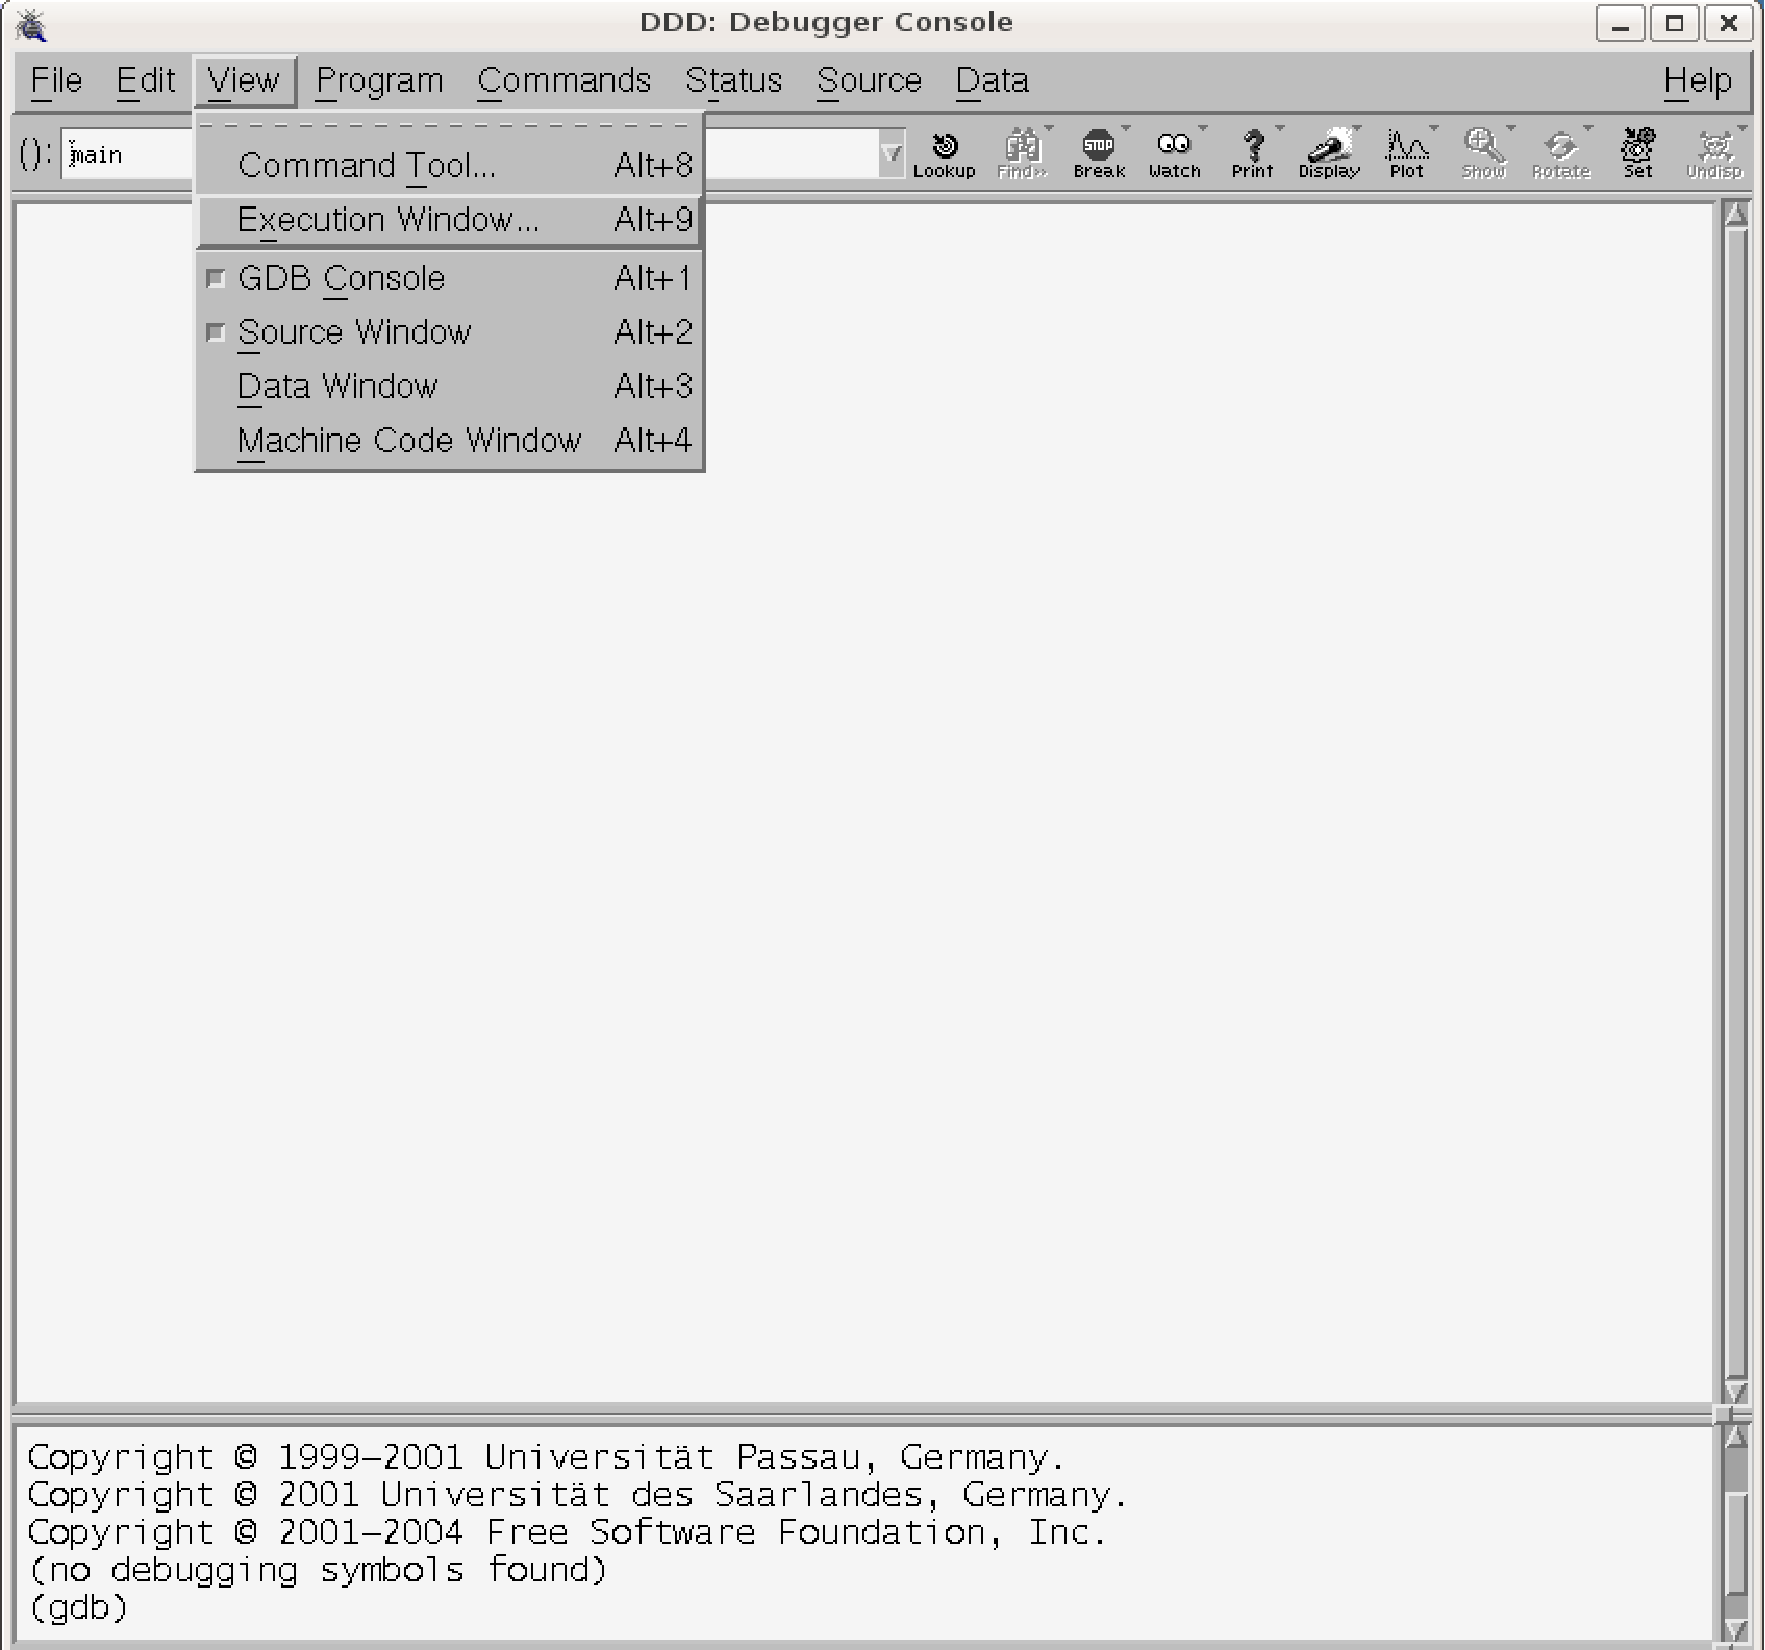
\includegraphics[width=8cm]{chapters/mardal-2/pdf/fig1.pdf}} \\
  \subfloat{ 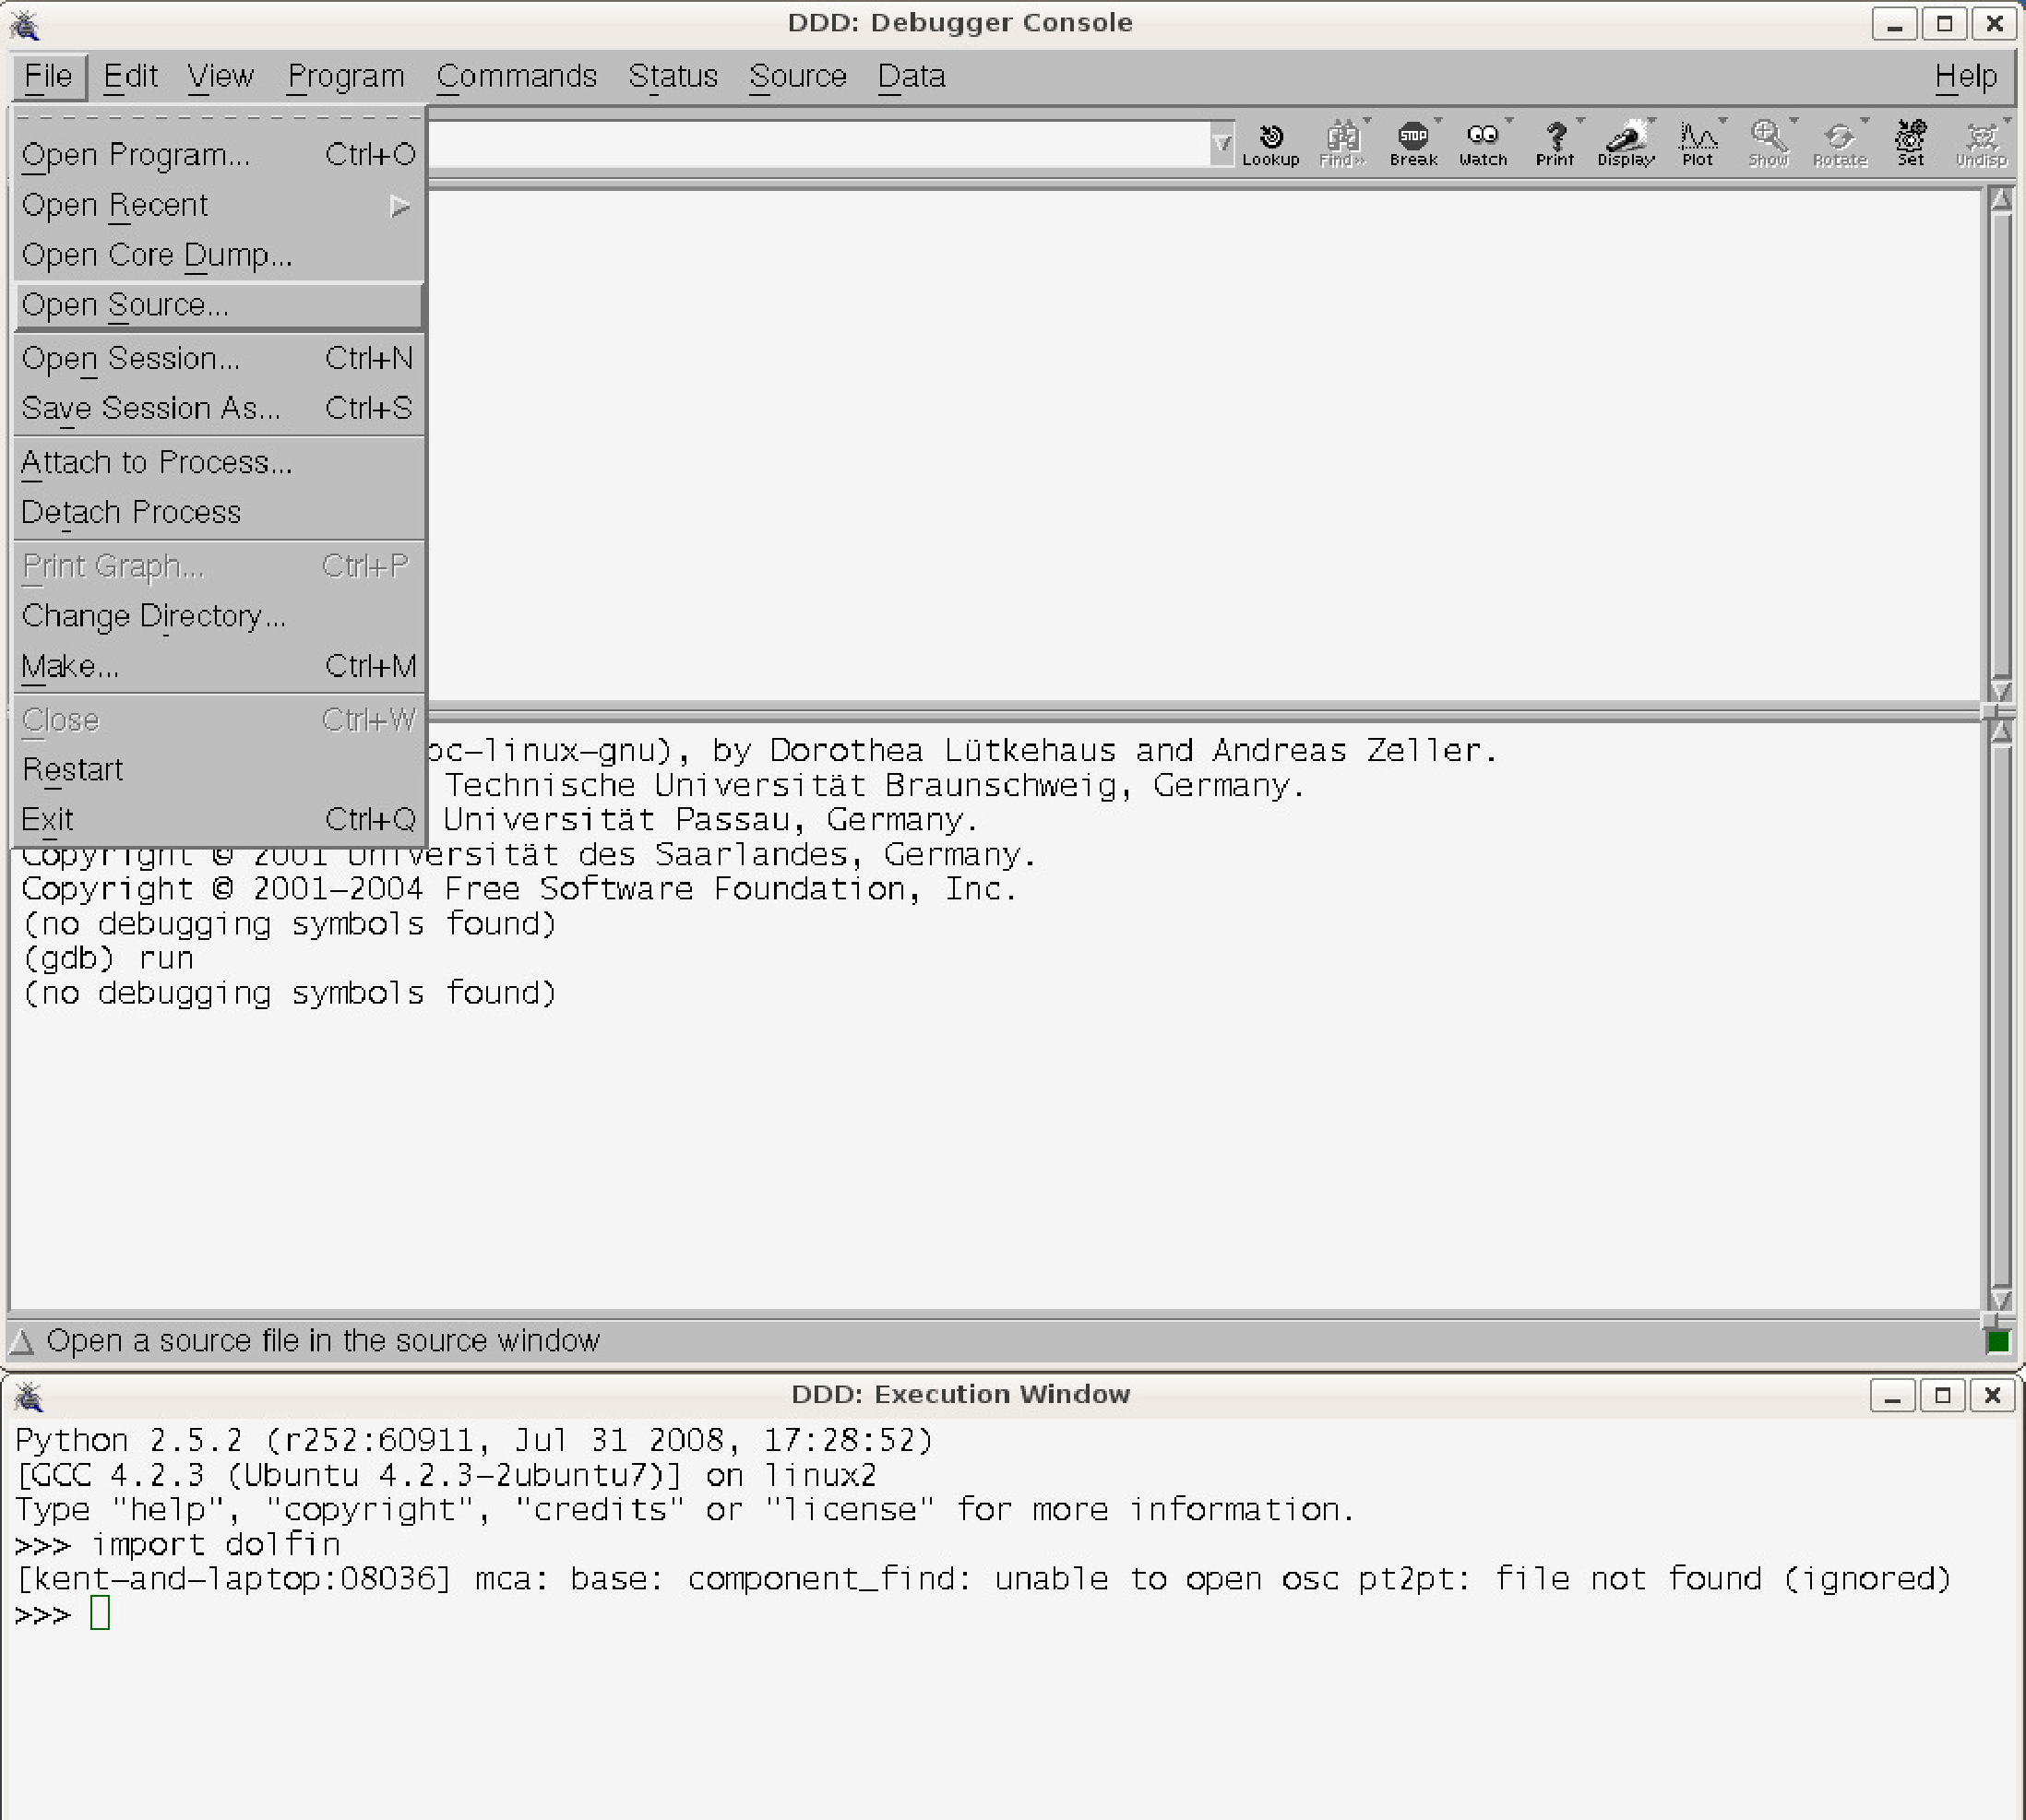
\includegraphics[width=8cm]{chapters/mardal-2/pdf/fig2.pdf}}
  \caption{Upper Picture: Starting a separate thread for the Python session in ddd.
           Lower Picture: Opening the source code after the \dolfin library has been loaded into Python.}
  \label{figure12}
\end{figure}
\begin{figure}
  \subfloat{ 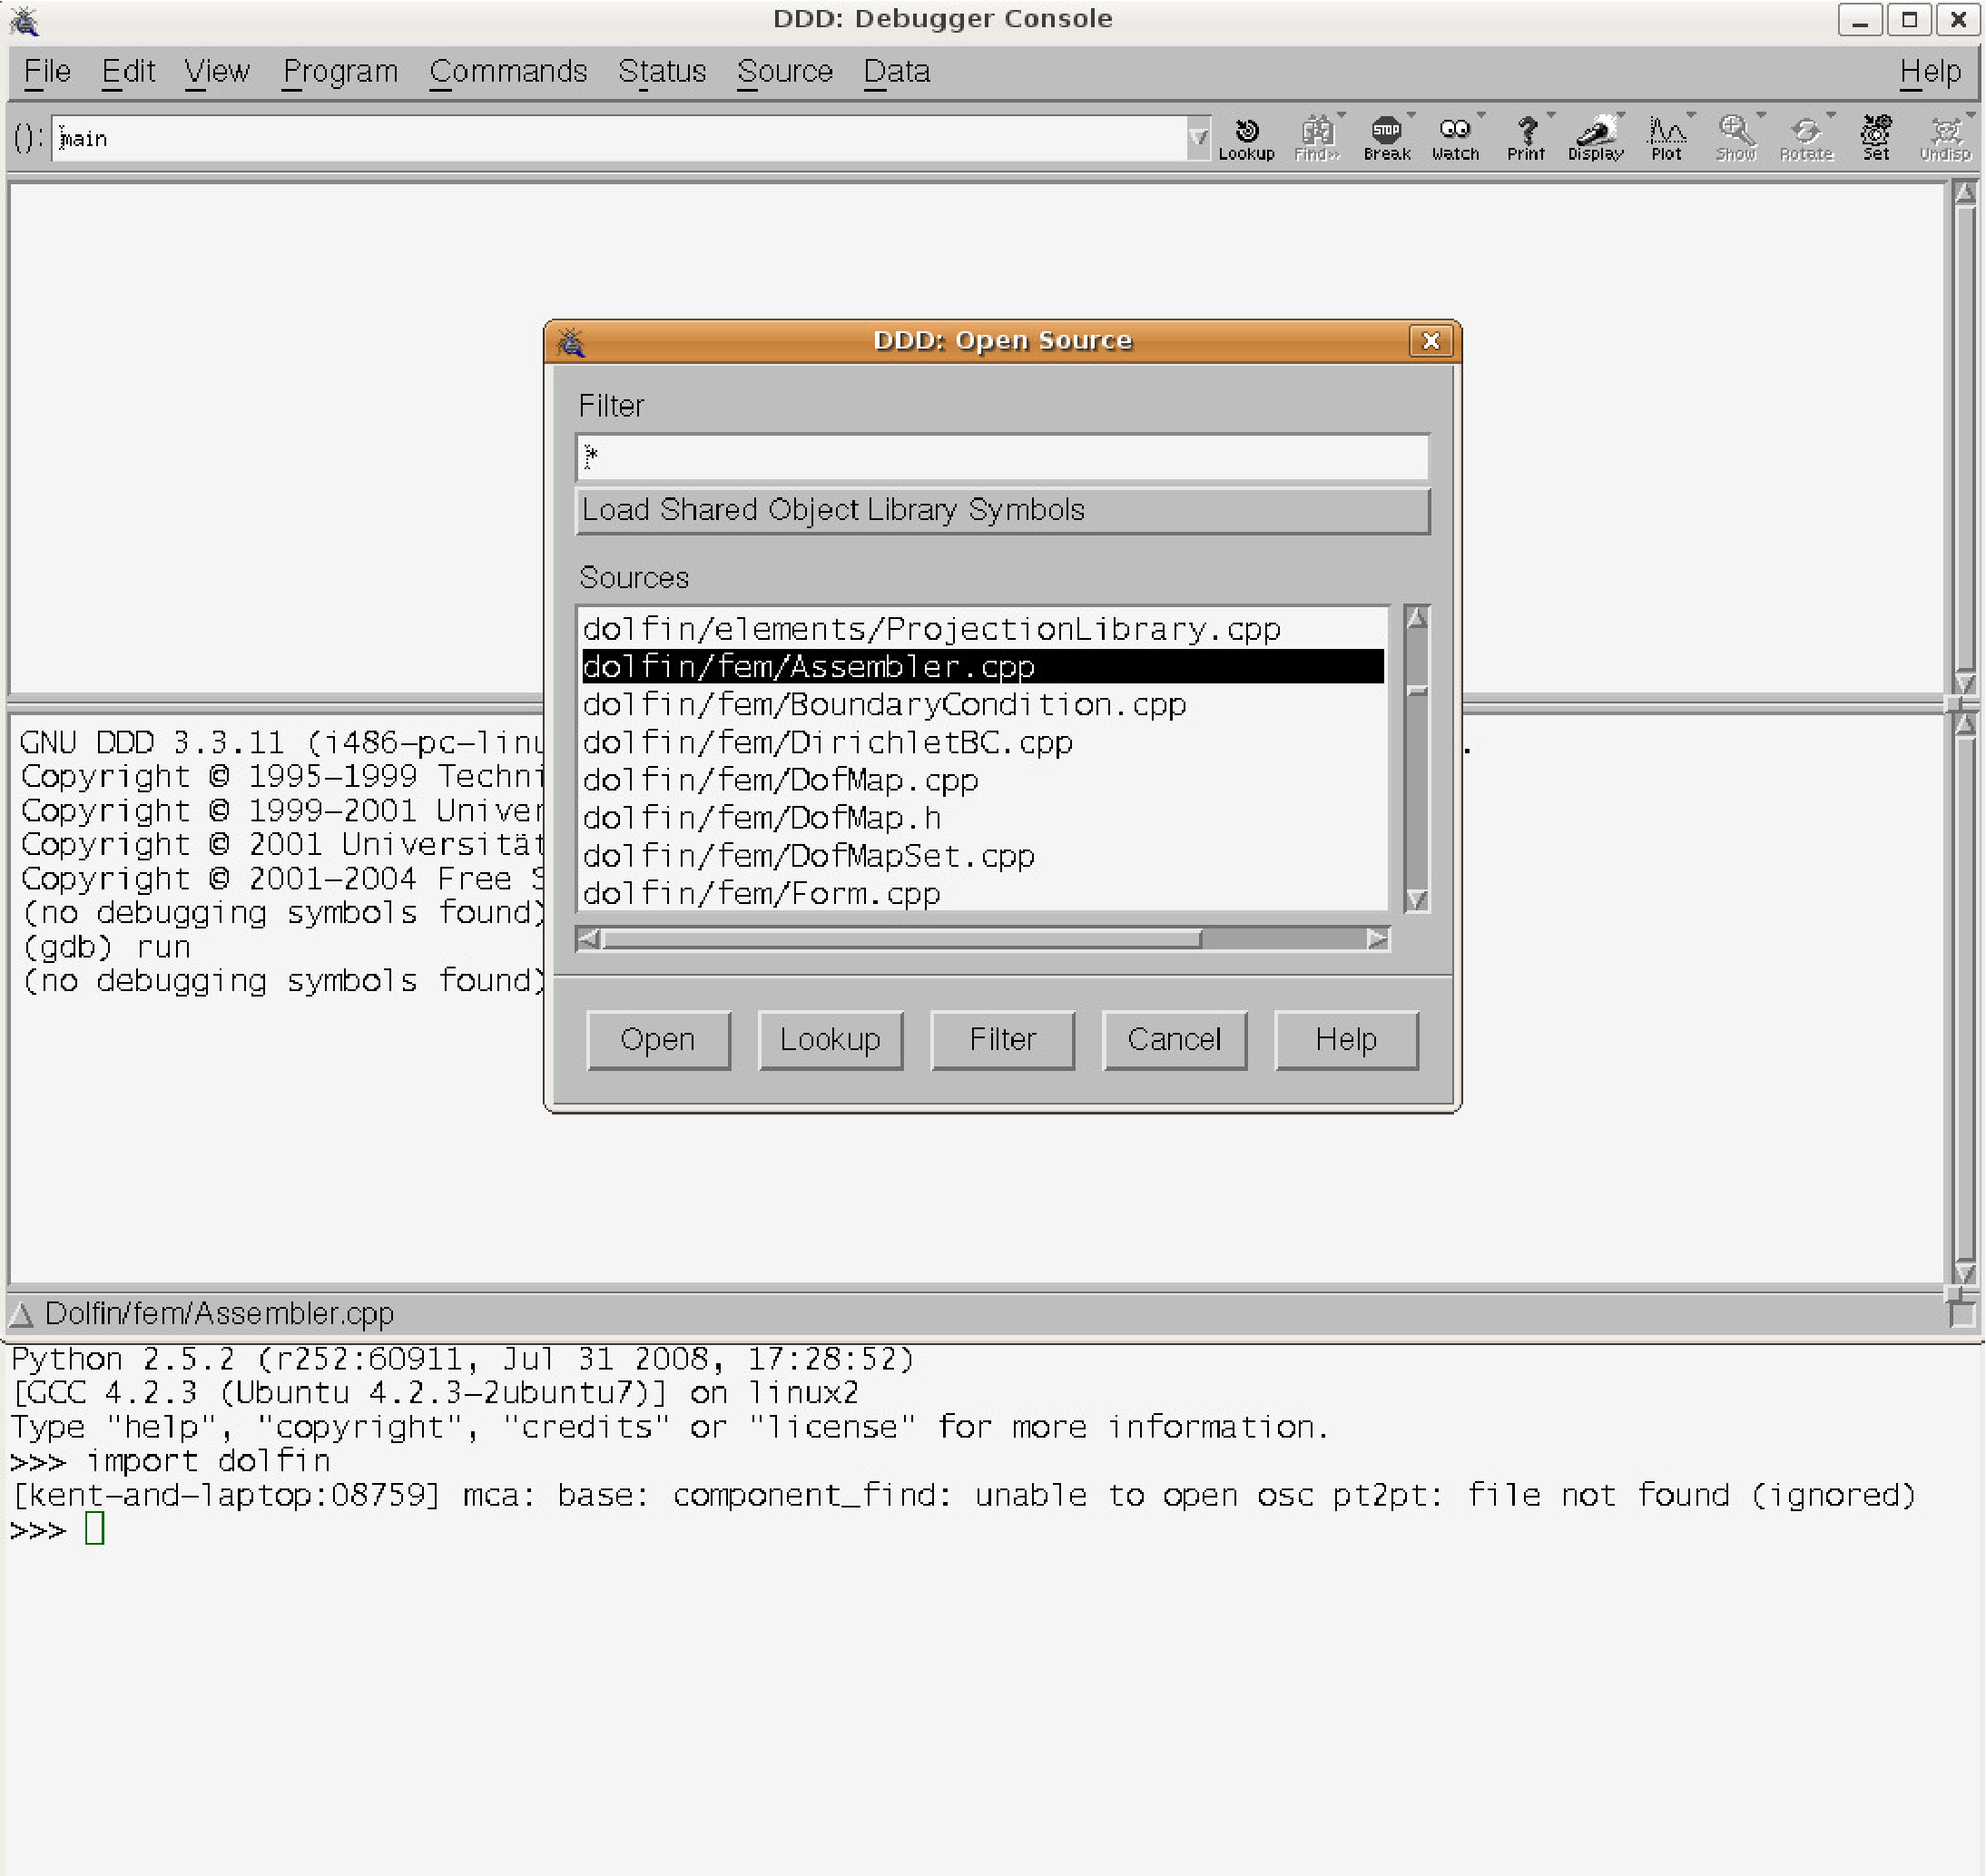
\includegraphics[width=8cm]{chapters/mardal-2/pdf/fig3.pdf}} \\
  \subfloat{ 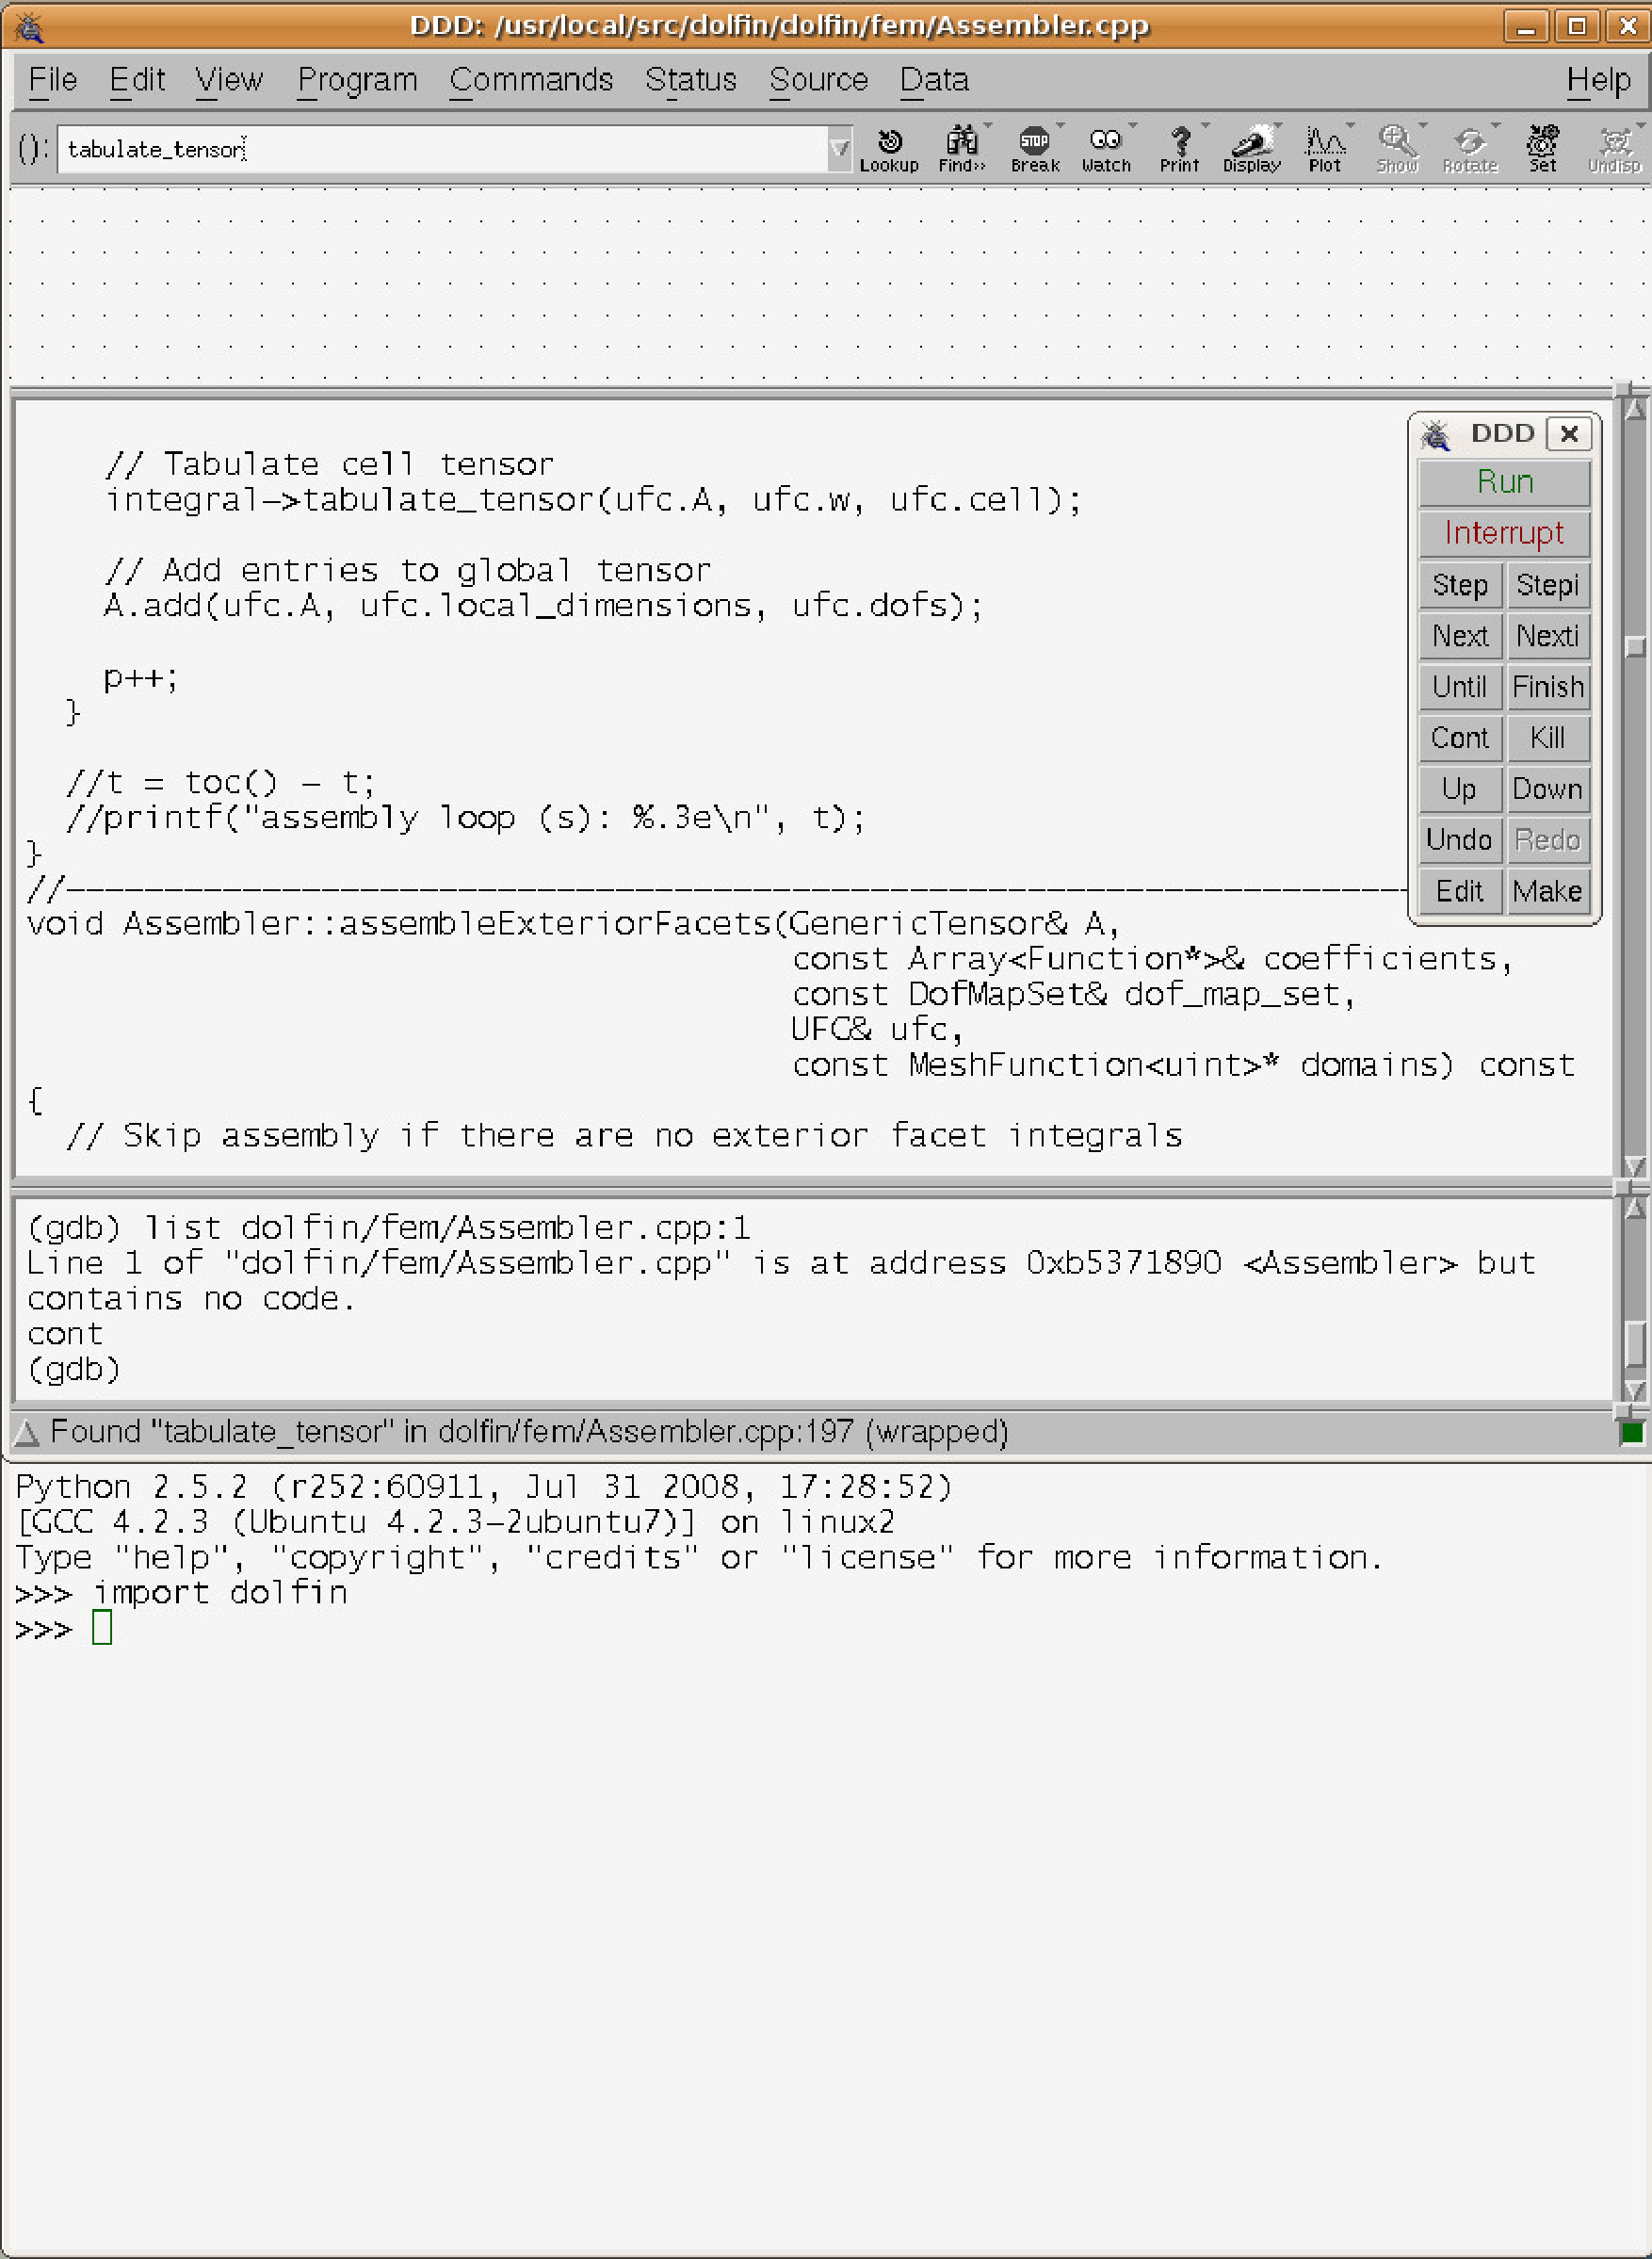
\includegraphics[width=8cm]{chapters/mardal-2/pdf/fig4.pdf}}
\caption{Upper Picture: Navigating through the source code for finding the assembly loop.
         Lower Picture: Searching for the function \emp{tabulate\_tensor.} }
\label{figure34}
\end{figure}

\begin{figure}
  \subfloat{ 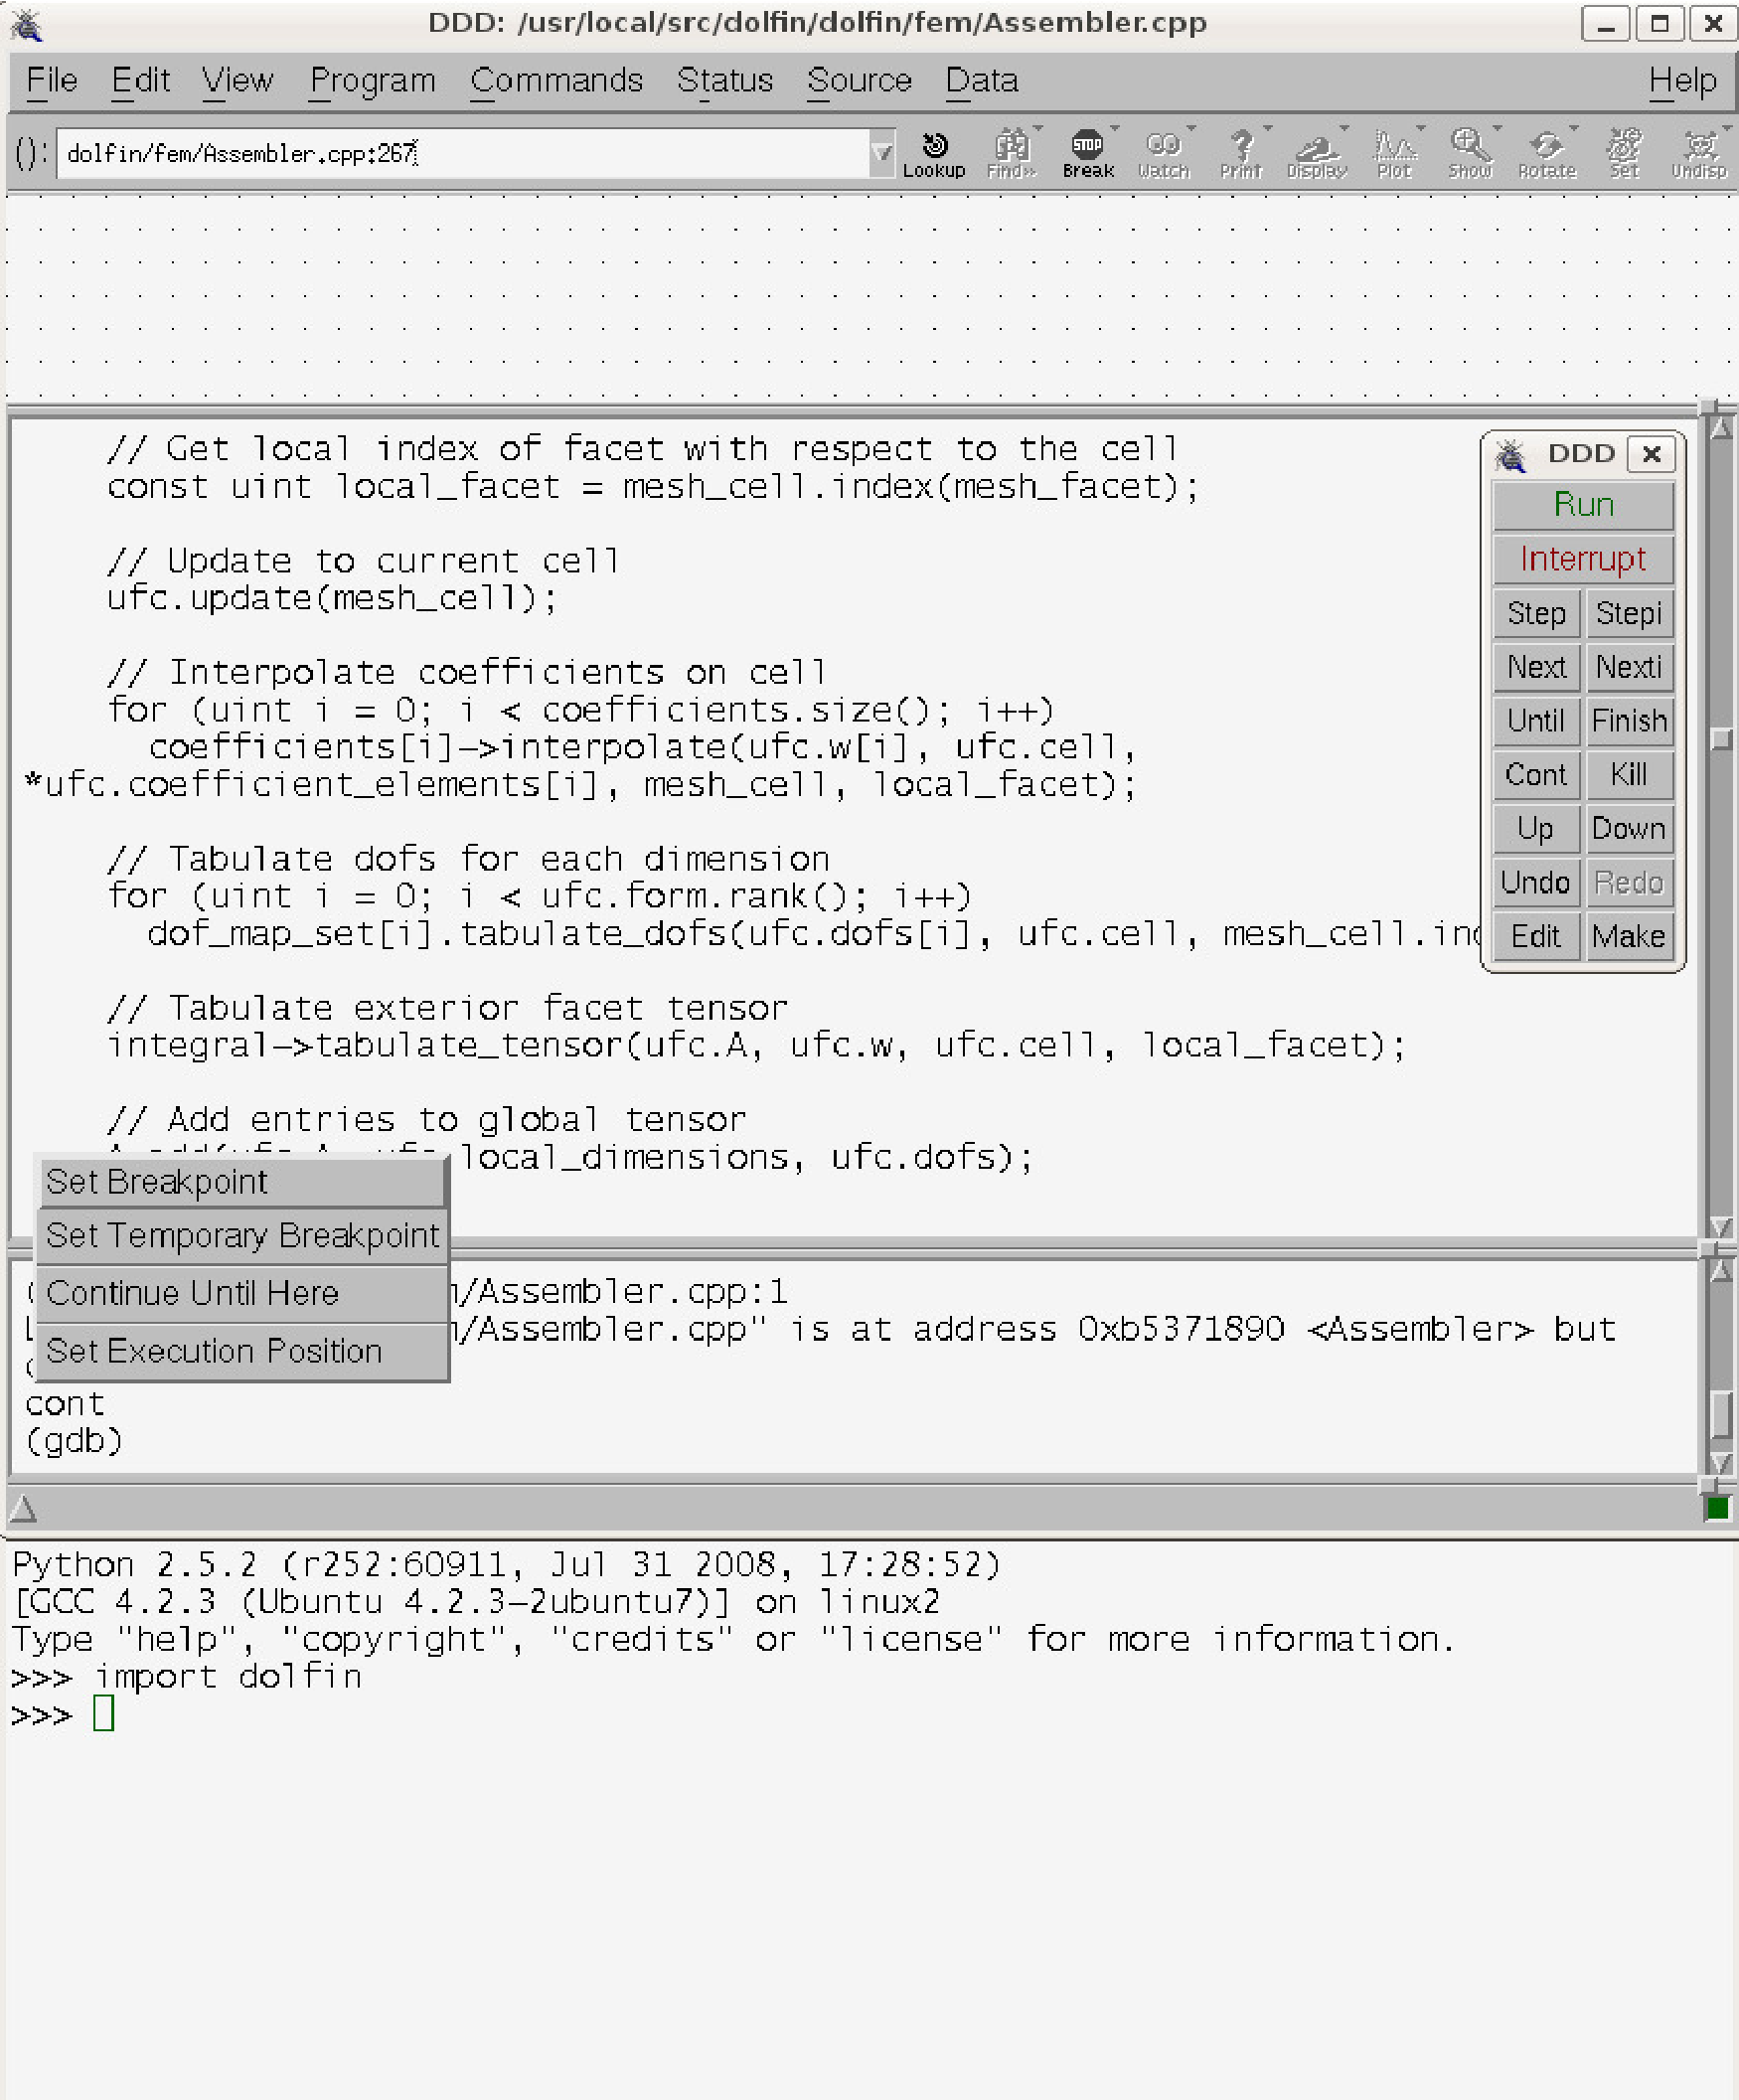
\includegraphics[width=8cm]{chapters/mardal-2/pdf/fig5.pdf}} \\
  \subfloat{ 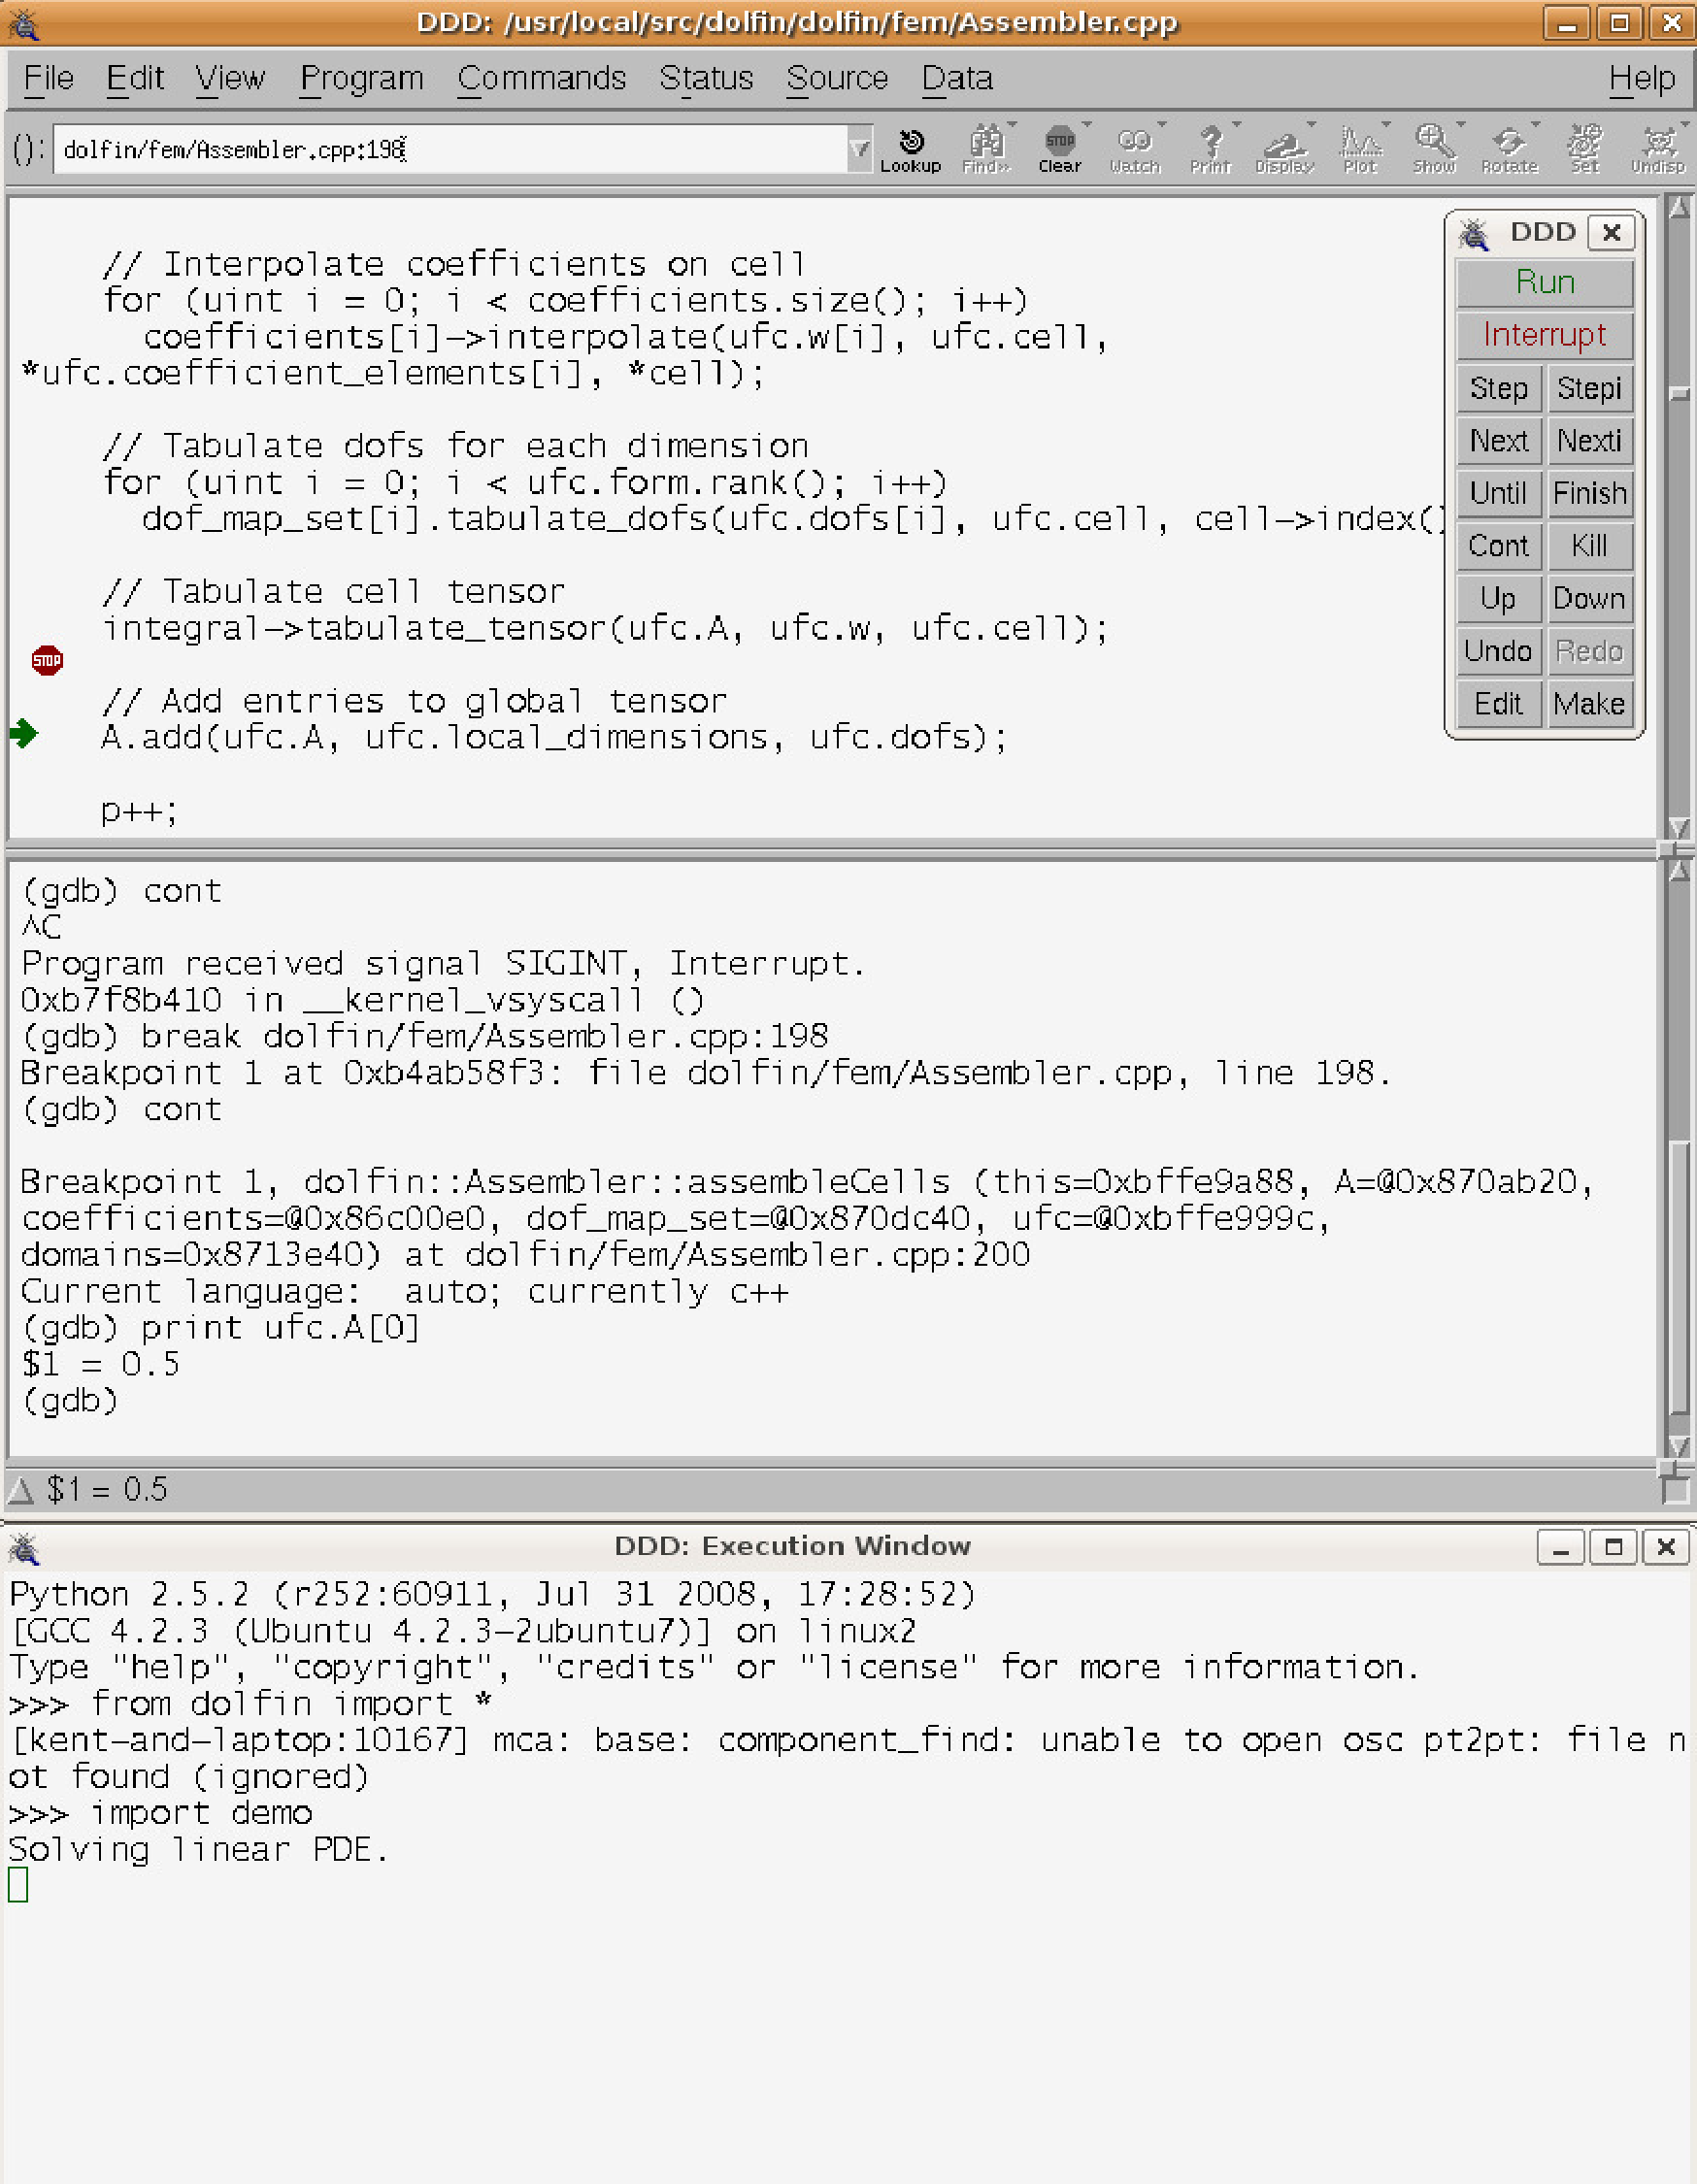
\includegraphics[width=8cm]{chapters/mardal-2/pdf/fig6.pdf}}
\caption{Setting a breakpoint after tabulate tensor and printing out the first element matrix entry.}
\label{fig5}
\end{figure}

\paragraph{Acknowledgments.}
The authors are very thankful to Johan Jansson who initiated the use of
SWIG to wrap \dolfin to Python. We are also thankful to Ola Skavhaug who
substantially extended the amount of \dolfin that got wrapped to Python and
to Martin Alnaes who contributed to the JIT compilations of
\emp{Expressions} and \emp{SubDomains}. 
Finally, Marie Rognes has improved the language in this chapter significantly. 

%%% Local Variables:
%%% mode: latex
%%% TeX-master: "../../book"
%%% End:
